\documentclass[12pt,a4paper]{article}

\input{../global_conf.tex}
\usepackage{epsdice}
\newtheorem{theorem}{Theorem}[section]
\newtheorem{definition}{Definizione}
\newtheorem{corollary}{Corollario}[theorem]
\newtheorem{lemma}[theorem]{Lemma}

\title{Appunti di Automi e linguaggi formali}
\author{Ejo Grejo}

\begin{document}

\maketitle
\tableofcontents
\newpage

\section{Introduzione}
\subsection{Problemi}
Per descrivere un \g{problema} bisogna specificare:
\begin{itemize}
	\item  Insieme dei possibili Input
	\item  Insieme dei possibili Output
	\item  La relazione tra Input e Output
\end{itemize}
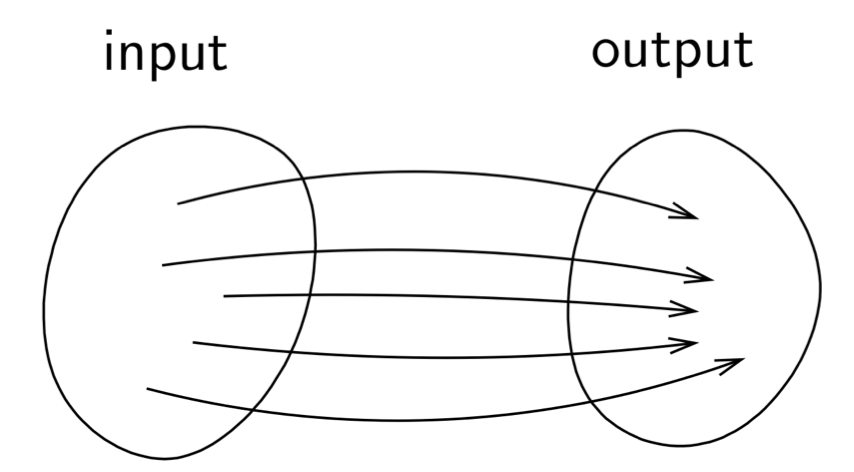
\includegraphics[scale=0.5]{img/funzione.png}

\nin\g{Algoritmo}: procedura meccanica che esegue delle computazioni (e può essere eseguita da un calcolatore).\\
Un algoritmo \g{risolve} un dato problema se:
\begin{itemize}
	\item Per ogni input, il calcolo dell'algoritmo si interrompe dopo un numero finito di passaggi.
	\item Per ogni input, l'algoritmo produce un output corretto.
\end{itemize}
\g{Correttezza} di un algoritmo:
Verificare che l'algoritmo risolva realmente il problema dato\\
\g{Complessità computazionale} di un algoritmo:
\begin{itemize}
	\item  \g{complessità temporale}: come varia il tempo di esecuzione rispetto alla dimensione dei dati di input
	\item  \g{complessità spaziale}: come varia la quantità di memoria utilizzata rispetto alla dimensione dei dati di input
\end{itemize}
\subsection{Linguaggi Formali}
\begin{itemize}
	\item Astrazione della nozione di problema
	\item I problemi sono espressi come \g{linguaggi} (insieme di stringhe) 
	\item Le soluzioni determinano se una determinata stringa è nell'insieme o no
		\begin{itemize}
			\item  Esempio: \textit{un certo intero $n$ è un numero primo?}
		\end{itemize}
	\item  Oppure, come \textit{trasformazioni tra linguaggi}
		\begin{itemize}
			\item Le soluzioni trasformano la stringa di input in una stringa di output
				\begin{itemize}
					\item Esempio: \textit{quanto fa $3+5$?}
				\end{itemize}
		\end{itemize}
\end{itemize}
Quindi in sostanza tutti i processi computazionali possono essere ridotti ad uno tra:
\begin{itemize}
	\item Determinazione dell'\textit{appartenenza} a un insieme (di stringhe)
	\item \textit{Mappatura} tra insiemi (di stringhe)
\end{itemize}
Formalizzeremo il concetto di computazione meccanica:
\begin{itemize}
	\item Dando una definizione precisa del termine "algoritmo"
	\item Caratterizzando i problemi che sono o non sono adatti per essere risolti da un calcolatore
\end{itemize}
\subsection{Automi}
Gli \textit{automi} sono dispositivi matematici astratti che possono:
\begin{itemize}
	\item Determinare l'appartenenza di una stringa ad un insieme di stringhe
	\item Trasformare una stringa in un'altra stringa
\end{itemize}
Hanno tutti gli \textit{aspetti} di un computer\\
Il tipo di \g{memoria} è cruciale:
\begin{itemize}
	\item memoria finita
	\item memoria infinita:
		\begin{itemize}
			\item con accesso limitato
			\item con accesso illimitato
		\end{itemize}
\end{itemize}
Abbiamo diversi tipi di automi per diversi classi di linguaggi\\
I diversi tipi di automi si differenziano per
\begin{itemize}
	\item La quantità di memoria (finita vs infinita)
	\item Il tipo di accesso alla memoria (limitato vs illimitato)
\end{itemize}
\newpage
\section{Linguaggi Regolari}
Un FA (NFA "[[Automi a Stati Finiti Non Deterministici]]" o DFA "[[Automi a Stati Finiti Non Deterministici]]) è un metodo per costruire una macchina che riconosce linguaggi regolari.\\
Un'\textit{espressione regolare} è un modo dichiarativo per descrivere un linguaggio regolare
Esempio: $$01* + 10*$$
Le espressioni regolari sono usate ad esempio in:
\begin{itemize}
	\item comandi UNIX (\textit{grep})
	\item strumenti per l'analisi lessicale di UNIX (\t{lex} \textit{Lexical analyzer generator}) e \t{flex} (\textit{Fast Lex})
	\item editor di testo
\end{itemize}
\subsection{Espressioni regolari}
sono costruite utilizzando:
\begin{itemize}
	\item un insieme di \textit{costanti} di base:
		\begin{itemize}
			\item $\epsilon$ per la stringa vuota
			\item $\varnothing$ per il linguaggio vuoto
			\item $a, b,...$ per i simboli $a,b,... \in \sum$
		\end{itemize}
	\item collegati da \textit{operatori}:
		\begin{itemize}
			\item $+$ per l'unione
			\item $.$ per la concatenazione
			\item $*$ per la chiusura di Kleene
		\end{itemize}
	\item Raggrupati usando le \textit{parentesi} $()$
\end{itemize}
Se $E$ è un espressione regolare, allora $L(E)$ è il \textit{linguaggio rappresentato da $E$}. La definizione di $L(E)$ è induttiva:
\begin{itemize}
	\item \g{Caso Base}:
		\begin{itemize}
			\item $L(\epsilon) = \{ \epsilon \}$
			\item $L(\varnothing) = \varnothing$
			\item $L(a) = \{a\}$
		\end{itemize}
	\item \g{Caso induttivo}:
		\begin{itemize}
			\item $L(E + F) = L(E) \cup L(F)$
			\item $L(EF) = L(E).L(F)$
			\item $L(E*) = L(E)^*$
			\item $L((E)) = L(E)$
		\end{itemize}
\end{itemize}
\g{Esempio}\\
$L=\{w \in \{0,1\}^* : 0$ e $1$ alternati in $w \}$\\
$(01)^* + (10)^* + 1(01)^* + 0(10)^*$ oppure $(\epsilon +1)(01)^*(\epsilon+0)$
\subsubsection{Precedenza}
Come per le espressioni aritmetiche, anche per le espressioni regolari ci sono delle \textit{regole di precedenza} degli operatori
\begin{enumerate}
	\item Chiusura di Kleene
	\item Concatenazione (punto)
	\item Unione
\end{enumerate}
\g{Esempio}\\
$01^*+1$ è raggruppato in $(0(1)^*)+1$\\
e denota un linguaggio \textit{diverso} da $(01)^*+1$
\subsection{Conversione per eliminazione di stati}
La procedura che vedremo è in grado di convertire un \textit{qualsiasi automa} (DFA o NFA) in un'{espressione regolare} equivalente.\\
Si procede per {eliminazione di stati}.\\
Quando uno stato $q$ viene eliminato i cammini che passano per $q$ scompaiono.\\
Si aggiungono nuove \textit{transizioni etichettate con espressioni regolari} che rappresentano i cammini eliminati.\\
Alla fine otteniamo un'espressione regolare che rappresenta \textit{tutti i cammini} dallo stato iniziale ad uno stato finale.\\
	$\rightarrow$ cioè il {linguaggio riconosciuto dall'automa}

\subsubsection{Da NFA a GNFA}
\mezzapagina
\begin{enumerate}
	\item Nuovo stato iniziale $q_{start}$ con transizione $\varepsilon$ verso il vecchio $q_0$ 
	\item Nuovo stato finale $q_{accept}$ con transizione $\varepsilon$ da tutti i vecchi stati finali $q\in F$ 
	\item Rimpiazzo transizioni multiple tra due stati con l'unione delle etichette
	\item Aggiungo transizioni etichettate con $\varnothing$ tra stati non collegati da transizioni
\end{enumerate}
\spazio
\begin{center}
	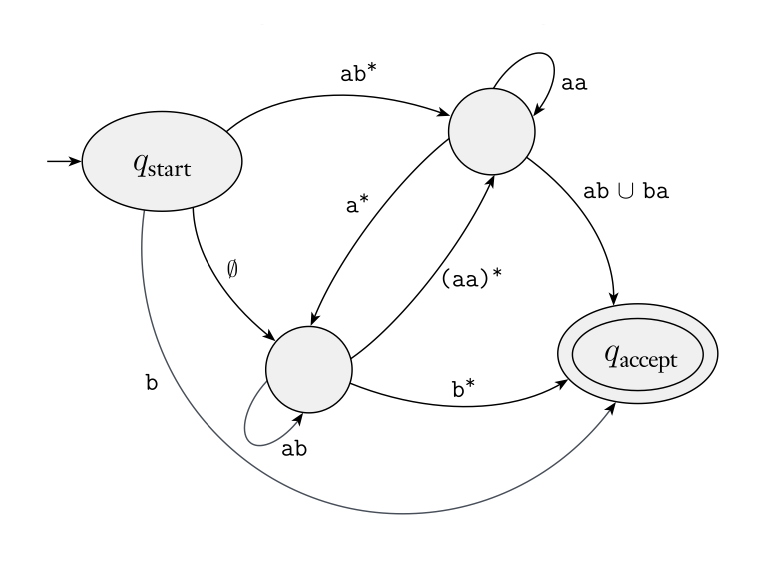
\includegraphics[scale=0.5]{img/NFAtoGNFA.png} 
\end{center}
\finemezzapagina
\subsection{Definizione formale di GNFA}
Un Automa a Stati Finiti Non Deterministico Generalizzato (GNFA) è una quintupla:
	$A=(Q, \sum, \delta, q_{start}, q_{accept})$
\begin{itemize}
	\item $Q$ è un insieme finito di \textit{stati}
	\item $\sum$ è un \textit{albero finito}
	\item $\delta : Q \backslash \{q_{accept}\} \times Q \backslash \mapsto R$ è una \textit{funzione di transizione} che prende in input \textit{2 stati} e restituisce 
		una \textit{espressione regolare} su $\sum$
	\item $q_{start} \in Q$ è lo \textit{stato iniziale}
	\item $q_{accept}$ è lo \textit{stato finale}
\end{itemize}
\subsubsection{Computazione di un GNFA}
Data una parola $w= w_1 w_2 ... w_m$ , dove $w_i \in \sum^*$
Una \textit{computazione} di un GNFA $A$ con input $w$ è una sequenza di stati $r_0r_1...r_m$ che rispetta \textit{2 condizioni}:
\begin{enumerate}
	\item $r_0 = q_{start}$ (inizia dallo stato iniziale)
	\item Per ogni $i, w_i \in L(R_i), dove R_i = \delta(r_{i-1}, r_i)$ (\textit{rispetta la funzione di transizione})
\end{enumerate}
Una computazione \textit{accetta} la parola $w$ se \textit{termina nello stato finale} ($r_m = q_{accept}$)\\\\
\mezzapagina
\begin{itemize}
	\item Partiamo da un GNFA con $k$ stati, dove $k\geq 2$ 
	\item Se $k>2$, eliminiamo uno stato $q_{rip}$ per ottenere un GNFA con $k-1$ stati.
	\item Quandk $k=2$, l'etichetta della transiione da $q_{start}$ a $q_{accept}$ è l'espressione regolare equivalente.
\end{itemize}
\spazio
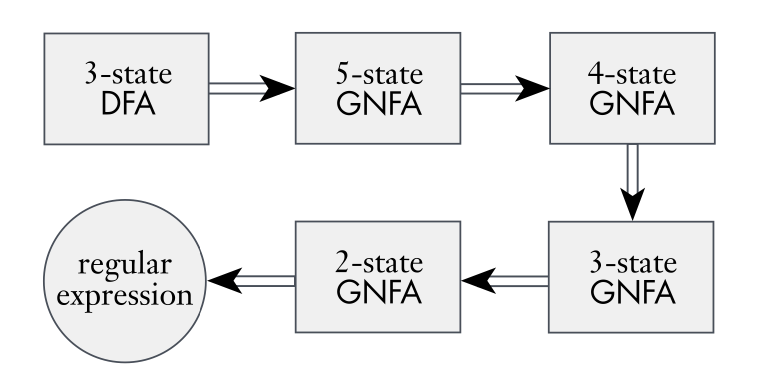
\includegraphics[scale=0.5]{img/GNFA_1.png}
\finemezzapagina

\mezzapagina
\begin{center}
	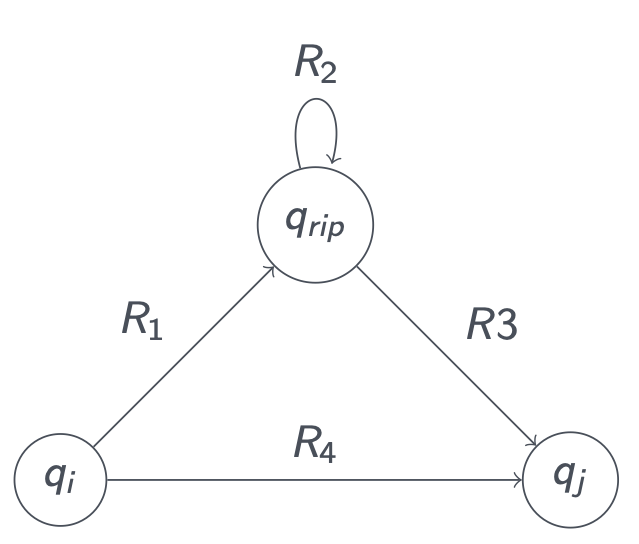
\includegraphics[scale=0.5]{img/GNFA_2.png}
\end{center}
\spazio
Se, nel GNFA:
\begin{enumerate}
	\item $q_i$ va in $q_{rip}$ con etichetta $R_1$ 
	\item $q_{rip}$ ha un self loop con etichetta $R_2$ 
	\item $q_{rip}$ va in $q_j$ con etichetta $R_3$ 
	\item $q_i$ va in $q_j$ con etichetta $R_4$ 
\end{enumerate}
\finemezzapagina

\mezzapagina
\begin{center}
	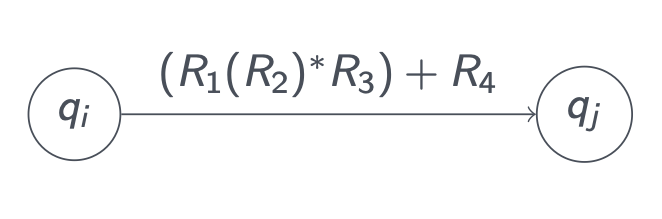
\includegraphics[scale=0.5]{img/GNFA_3.png}
\end{center}
\spazio
dopo l'eliminazione di $q_{rip}$, $q_i$ va in $q_j$ con etichetta 
$$(R_1(R-2)*R_3)+R_4$$
\finemezzapagina

\paragraph{Algoritmo di conversione}
\t{Convert(A)}
\begin{enumerate}
	\item Sia $k$ il numero di stati di $A$
	\item Se $k=2$, ritorna l'espressione $R$ che collega $q_{start}$ con $q_{accept}$
	\item Se $k > 2$, scegli $q_{rip} \in Q \backslash \{q_{start}, q_{accept}\}$ e costruisci un GNFA $A' = (Q',\sum, \delta ', q_{start}, q_{accept})$ come segue:
		\begin{itemize}
			\item $Q' = Q \backslash \{q_{rip}\}$
			\item per ogni $q_i \in Q' \backslash \{q_{accept}\}, q_j \in Q' \backslash \{q_{start}\}$, sia $\delta '(q_i,q_j) = (R_1(R_2)*R_3)+R_4$ 
		\end{itemize}
	 	 dove $R_1 = \delta (q_i,q_{rip}), R_2 = \delta (q_{rip}, q_{rip}), R_3 = \delta (q_{rip}, q_j)$ e $R_4=\delta (q_i, q_j)$
	 \item Ritorna il risultato calcolato da \t{Convert(A')}
\end{enumerate}

\newpage
\section{Linguaggi Non Regolari}
Di quanti stati necessita l'automa che riconoscere linguaggio $\{0^n1^n|n\geq0\}$?
Occorrono $2n$ stati per poter riconoscere il linguaggio. Essendo $n$ infinito non è possibile 
determinare un numero finito di stati, pertanto il linguaggio $\{0^n1^n|n\geq0\}$ non è regolare, 
proprio perché non può essere riconosciuto da un automa a stati finiti. 

\paragraph{Dimostrazione}

È necessario ragionare \textit{per assurdo}, in quanto siamo costretti a dimostrare che non esiste un automa 
a stati finiti che riconosce un linguaggio che ipotizziamo essere non regolare. 
Supponiamo che  $L_{01}=\{0^n1^n|n\geq0\}$ sia regolare, allora esiste un DFA $A$ che accetta $L_{01}$ con $k$ stati. 
Cerchiamo ora di dimostrare che esiste una parola appartenente a $L_{01}$ che non viene riconosciuta dall'automa DFA.
L'automa segue una computazione $r_0, r_1, r_2,\dots,r_k$ ovvero di lunghezza $k+1$, questo comporta che 
all'interno della sequenza c'è uno stato che si ripete, supponiamo che si tratti di  $r_i =r_j$ per qualche $a$.
Posso sfruttare questo fatto per far sbagliare l'automa:
considero la parola $0^i1^i$, la computazione ha la forma $$r_0, r_1, \dots, r_i, s_1, \dots, s_i$$
$s_i$ è uno stato finale? Sì, $s_i$ deve essere finale. 
Cosa succede se a questo automa forniamo in input la parola $0^j1^i$ ? 
Abbiamo detto che $r_j=r_i$ quindi l'automa terminerà nello stesso stato finale $s_i$ e 
dunque verrebbe riconosciuta una parola che non appartiene a $L_{01}$.

\subsection{SBRODEGHI}
\begin{itemize}
	\item supponiamo che $l_{0}=\{0^n1^n | n \geq 0\}$ 
	\item ...

	\item cosa succede quando l; automa $A$ legge $1^i$ partendo da $q$ 
	\item se l'automa finisce la lettura in uno stato finale
		\item allora accetta, sbagliando la parola $0^j1^j$ 
	\item se l'automa finisce la lettura in uno stato non finale
		\item allora rifiuta sbagliando la parola $0^i1^i$ 
	\item in entrambi i casi abbiamo ingannato l'automa, quindi $L_{01}$ *non può essere regolare*
\end{itemize}

\subsubsection{Proprietà dei linguaggi regolari}
Possono essere utilizzate per dimostrare che un DFA effettua un loop per accettare un linguaggio regolare.
La dimostrazione è più facile rispetto a quella precedente. 
\subsection{Pumping Lemma}
Sia $L$ un linguaggio regolare. Allora
\begin{itemize}
	\item  \g{esiste una lunghezza} $k>0$ tale che 
	\item  \g{ogni parola} $w\in L$ di lunghezza $|w|\geq k$ 
	\item  \g{può essere spezzata} in $w =xyz$ tale che 
\end{itemize}
\begin{enumerate}
	\item $y\neq \varepsilon$ (il secondo pezzo è non vuoto)
	\item $|xy|\leq k$ (i primi due pezzi sono lunghi al max $k$)
	\item $\forall i \geq 0, xy^iz\in L$ (possiamo "pompare" $y$ rimandandolo in $L$)
\end{enumerate}
\subsubsection{Dimostrazione}
\begin{itemize}
	\item Supponiamo che $L$ sia un linguaggio regolare
	\item Allora è riconosciuto da un DFA con, supponiamo, $k$ stati
	\item Consideriamo una parola $w = a_1, a_2, \dots, a_n\in L$ di lunghezza $n\geq k$ 
	\item Consideriamo gli stati nella computazione di $A$ per $w$ 
\end{itemize}
$$p_0, p_1, p_2,\dots p_k\dots p_n$$
Siccome in $p_0, p_1,\dots p_k$ ci sono $k+1$ stati ne esiste uno che si ripete:\\
Esistono $l< m$ tali che $p_l=p_m$ e $m \leq k$ 

\subsubsection{Pumping lemma come gioco} 
Esiste una strategia che ci consente di vincere sempre su un certo linguaggio. 
\begin{enumerate}
	\item $\exists k>o$  (giocatore 1 sceglie la dimensione di $k$)
	\item $\forall w\in L, |w|\geq k$ (giocatore 2 sceglie una parola)
	\item $\exists xyz\mid w= xyz$
		$y\neq \varepsilon$ 
		$|xy| \leq k$ (giocatore 1 sceglie come partizionare la parola)
	\item	$\forall i\geq 0 xy^iz\in L$ (giocatore 2 sceglie una potenza affinché la condizione sia verificata)
\end{enumerate}
Se giocatore 2 vince allora il linguaggio non è regolare. 

\subsubsection{Esistono linguaggi non regolari che rispettano il Pumping Lemma}

\paragraph{Sia $L_{ab}$ il linguaggio delle stringhe sull'alfabeto $(a,b)$ dove il numero di $a$ è uguale al numero di $b$. $L_{ab}$ è regolare?}\nin
Per assurdo ipotizzo $L_{ab}$ regolare. \\
Se lo è, allora rispetta il Pumping Lemma $\rightarrow$ deve esistere una lunghezza $k>0$ che rende vero il Pumping Lemma.\\
Consideriamo la parola $w=a^kb^k$ , $w$ appartiene al linguaggio e $|w|>k$.\\
Per ogni suddivisione $w\in xyz$ dove $y\neq \varnothing$ e $|xy|\leq k$ \\
$$x = a^P$$
$$y = a^Q$$
$$z = a^{K-P-Q}b^K$$
Se prendiamo come esponente $i=2$ , $xy^2z=a^Pa^{2Q}a^{K-P-Q}b^K= a^{Q+K}b^K$ la parola non fa parte del linguaggio.\\
\g{Conclusione: per assurdo non è regolare.}\\

\paragraph{Il linguaggio $L_{rev} = \{ww^R:w \in\{a,b\}*\}$ è regolare?}\nin\\

$w^R = w$ scritto alla rovescia

$w = w_1, w_2, \dots, w_k$ 

$w^R=w_n, w_{n-1}, \dots, w_1$ 
\begin{enumerate}
	\item Suppongo $L_{rev}$ sia regolare,allora esiste $k>0$ che rende vero il Pumping Lemma
	\item considero la parola $w=a^kb^2a^k$ 
	\item Per ogni suddivisione di $xyz$ dove $y\neq \varepsilon$ e $|xy|\leq k$ 
\end{enumerate}
$$x = a^P$$
$$y = a^Q$$
$$z = a^{K-P-Q}b^2a^K$$
Se prendiamo come esponente $i=2$ , $xy^2z=a^Pa^{2Q}a^{K-P-Q}b^2a^K= a^{Q+K}b^2a^K$ la parola non fa parte del linguaggio.\\
\g{Conclusione: per assurdo non è regolare.}


\paragraph{Il linguaggio $L_{p} = \{1^p: p$  è primo$\}$ è regolare?}\nin
\begin{enumerate}
	\item Assumo che $L_p$ sia regolare e che $k>0$ sia la lunghezza che rende vero il Pumping Lemma. 
	\item Considero $w=1j$ dove $j$ è il primo numero primo $>k$ 
	\item Per ogni suddivisione $w=xyz$ dove $y\neq \varnothing$ e $|xy| \leq k$ 
		\begin{enumerate}
			\item $x=1^P$ 
			\item $y = 1^Q$ 
			\item $z=1^{J-P-Q}$ dove $Q>0$ e $P+Q \leq k$ 
		\end{enumerate}
\end{enumerate}

$i=2$ \\
$xy^2z = 1^P1^{2Q}1^{J-P-Q}=1^{Q+J}$\\
\\
$i=2J$\\
$xy^{2J}z = 1^P1^{2jQ}1^{J-P-Q}=1^{(2J)Q+J-Q}$\\
$= 1^{(2J-1)Q+J} = 1^{(Q+1)J} \not\in L_p$ \\
La parola non è contenuta nel linguaggio in quanto la sua lunghezza è un numero scomponibile in fattori. 


\newpage
\section{Linguaggi Context-Free}
Abbiamo visto che esistono \textit{linguaggi non regolari} (ad esempio $\{0^n1^n | n\geq 0\}$),
Consideriamo ora una classe più grande di linguaggi, i \g{Linguaggi Context-free (CFL)},
usati nello studio dei linguaggi naturali dal 1950, e nello studio dei compilatori dal 1960.
Vedremo dunque due metodi per descrivere un linguaggio CFL:
\begin{itemize}
	\item Grammatiche Context-free
		% link automi a pila
	\item Automi a pila (pushdown automata)
\end{itemize}

\subsection{Grammatiche Context-free}
Le grammatiche context-free sono un metodo più potente per descrivere i linguaggi, 
si prestano particolarmente bene a descrivere comportamenti ricorsivi all'interno di un linguaggio. \\
Inizialmente sono state utilizzate per descrivere i \g{linguaggi naturali} 
%link grammatica per l'inglese
(vedi Una grammatica per l’inglese), 
oggi sono fondamentali per lo sviluppo dei *parser*.

Vediamo ad esempio la grammatica $G_1$:

$$A\rightarrow 0A1$$
$$A\rightarrow B$$
$$B\rightarrow \#$$
Quello che possiamo notare è la presenza di 
\begin{itemize}
	\item un insieme di \g{regole di sostituzione} (o \textit{produzioni})
	\item alcune \g{variabili} ($A$ e $B$ )
	\item i \g{terminali} ossia i simboli dell'alfabeto ($0,1,\#$)
	\item una \g{variabile iniziale} $A$ 
\end{itemize}
\begin{enumerate}
	\item Scrivi la variabile iniziale
	\item Trova una variabile che è stata scritta e una regola che inizia con quella variabile.
		Sostituisci la variabile con il lato destro della regola. 
	\item Ripeti 2. fino a quando non ci sono più variabili.
\end{enumerate}

\paragraph{Esempio per $G_1$}
$$A\Rightarrow 0A1\Rightarrow 00A11 \Rightarrow 000A111\Rightarrow 000\#111$$
La sequenza di sostituzioni si chiama \g{Derivazione di 000\#111}

\subsection{Albero sintattico}
Una derivazione definisce un \g{albero sintattico (parse tree)}\\
\begin{center}
	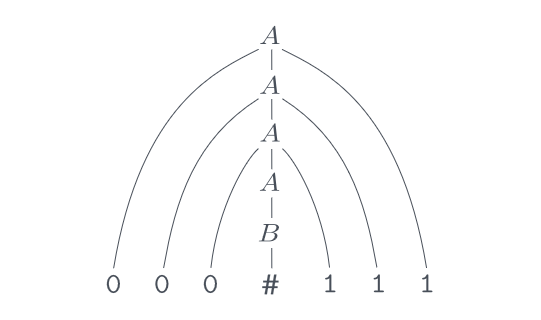
\includegraphics[scale=0.5]{img/alberosintattico.png} 
\end{center}
\begin{itemize}
	\item la radice è la variabile iniziale
	\item i nodi interni sono variabili 
	\item le foglie sono terminali 
\end{itemize}

Tutte le stringhe generate in questo modo costituiscono il *linguaggio della grammatica* $G_1$, ossia $L(G_1)$. 

\subsection{Una grammatica per l’inglese}
Definiamo $G_2$ nel seguente modo: \\
$\langle SENTENCE \rangle \rightarrow \langle NOUN$-$PHRASE\rangle \langle VERB$-$PHRASE \rangle$\\
$\langle NOUN$-$PHRASE\rangle \rightarrow \langle CMPLX$-$NOUN\rangle$\\
$\langle NOUN$-$PHRASE\rangle  \rightarrow \langle CMPLX$-$NOUN \rangle \langle PREP$-$PHRASE \rangle$ \\
$\langle VERB$-$PHRASE \rangle  \rightarrow \langle CMPLX$-$VERB \rangle$\\
$\langle VERB$-$PHRASE \rangle  \rightarrow \langle CMPLX$-$VERB \rangle \langle PREP$-$PHRASE \rangle$\\
$\langle PREP$-$PHRASE \rangle  \rightarrow \langle PREP\rangle\langle CMPLX$-$NOUN \rangle$\\
$\langle CMPLX$-$NOUN \rangle → \langle ARTICLE \rangle \langle NOUN\rangle$\\
$\langle CMPLX$-$VERB \rangle → \langle VERB\rangle | \langle VERB\rangle \langle NOUN$-$PHRASE\rangle$\\
$\langle ARTICLE \rangle \rightarrow$  \t{a | the}\\
$\langle NOUN\rangle\rightarrow$  \t{boy | girl | flower}\\
$\langle VERB\rangle\rightarrow$ \t{touches | likes | sees}\\
$\langle PREP\rangle\rightarrow$ \t{with}\\

\nin La grammatica $G_2$ ha 10 variabili ($SENTENCE$ , $NOUN$-$PHRASES$, eccetera...), 27 terminali, 
ovvero i simboli dell'alfabeto inglese standard, e 18 regole. Tra le stringe di $L(G_2)$ vi sono \\

	\t{a boy sees}
	
	\t{the boy sees a flower}
	
	\t{a girl with a flower likes the boy}\\
	\\
Ognuna di queste stringhe ha una derivazione nella grammatica $G_2$, ad esempio \\
$\langle SENTENCE \rangle \rightarrow \langle NOUN$-$PHRASE\rangle \langle VERB$-$PHRASE \rangle$

$\rightarrow\langle CMPLX$-$NOUN\rangle \langle VERB$-$PHRASE \rangle$

$\rightarrow  \langle ARTICLE \rangle \langle NOUN\rangle \langle VERB$-$PHRASE \rangle$

$\rightarrow$ \t{a} $\langle NOUN\rangle\langle VERB$-$PHRASE\rangle$

$\rightarrow$ \t{a boy} $\langle VERB$-$PHRASE\rangle$

$\rightarrow$ \t{a boy} $\langle CMPLX$-$VERB\rangle$

$\rightarrow$ \t{a boy} $\langle VERB\rangle$

$\rightarrow$ \t{a boy sees}
			

\subsection{Definizione di grammatica context-free}
Una grammatica context-free è una quadrupla $(V,\Sigma,R,S)$ dove 
\begin{itemize}
	\item $V$ è un insieme finito di \g{variabili}
	\item $\Sigma$ è un insieme finito di \g{terminali} disgiunto da $V$ 
	\item $R$ è un insieme di \g{regole}, dove ogni regola è una variabile e una stringa di variabili e terminali 
	\item $S\in V$ è la \g{variable iniziale}
\end{itemize}
Se $u, v , w$  sono stringhe di variabili e terminali e $A \rightarrow w$ è una regola:
\begin{itemize}
	\item $uAv$  \g{produce} $uwv : uAv \Rightarrow uwv$ 
	\item $u$ \g{deriva} $v : u \Rightarrow^* v$ se:
		\begin{itemize}
			\item $u = v$  , oppure
			\item esiste una sequenza $u1, u2, \dots, uk$ tale che
				$u \Rightarrow u1 \Rightarrow u2 \Rightarrow \dots \Rightarrow uk \Rightarrow v$
				$\Rightarrow$ 
		\end{itemize}
	\item il \g{linguaggio della grammatica} è $L(G) = \{w \in \Sigma^* \mid S \Rightarrow^* w \}$
\end{itemize}

\subsection{Esempi}
\subsubsection{Parentesi}
Consideriamo la grammatica $G_3 = \langle \{S\}, \{a,b\}, R, S\rangle$.  L'insieme delle regole della grammatica $G_3$ , ossia $R$, è
$$S\rightarrow aSb \mid SS \mid \varepsilon$$
Questa grammatica genera stringhe come 
\begin{itemize}
	\item \t{abab}: $S\rightarrow SS\rightarrow abS \rightarrow abab$ 
	\item \t{aaabbb} $S\rightarrow aSb\rightarrow aaSbb \rightarrow aaaSbbb\rightarrow aaabbb$ 
	\item \t{aababb}: $S\rightarrow aSb\rightarrow aSSb\rightarrow aabSb\rightarrow aababb$ \\
\end{itemize}
Si può più dedurre più facilmente di che linguaggio si tratta pensando ad \t{a} come ad una parentesi aperta "(" e a \t{b}
come ad una parentesi chiusa ")". \\
Visto in questo modo, $L(G_3)$ è il linguaggio di tutte le stringhe di \g{parentesi correttamente annidate}.\\
Si osservi che il lato destro di una regola può essere la parola vuota $\varepsilon$ 

\subsubsection{Operazioni aritmetiche}
Si consideri la grammatica $G_4 = (V,\Sigma, R, \langle EXPR \rangle)$\\
$V$ è $\{\langle EXPR \rangle, \langle TERM \rangle, \langle FACTOR \rangle\}$ e $\Sigma$ è $\{a, +, \times, (,)\}$ \\
Le regole sono: \\
	
	$\langle EXPR \rangle \rightarrow \langle EXPR \rangle + \langle  TERM\rangle \mid \langle  TERM\rangle$
	
	$\langle TERM \rangle \rightarrow \langle TERM\rangle \times \langle FACTOR\rangle \mid \langle FACTOR \rangle$ 
	
	$\langle FACTOR\rangle \rightarrow (\langle EXPR\rangle) \mid a$\\
\\
Le due stringhe \t{a+axa} e \t{(a+a)xa} possono essere generate dalla grammatica $G_4$, e questi sono i loro alberi sintattici. \\
\begin{center}
	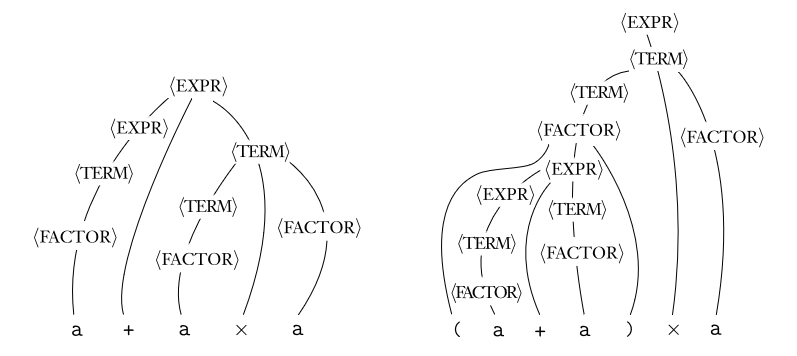
\includegraphics[scale=0.5]{img/alberi_g_4.png}
\end{center}
\subsection{Come si progetta una grammatica context-free}
Abbiamo appena visto la grammatica $G_4$. Tale grammatica potrebbe benissimo costituire una sottogrammatica
di un \textit{linguaggio di programmazione}, in quanto le operazioni aritmetiche sono una componente 
fondamentale dei linguaggi di programmazione. \\
In questo e in altri svariati contesti è probabile imbattersi in una CFG (context-free grammatic) composta da altre grammatiche meno complesse.
Per unire queste grammatiche è necessario creare una regola 
$S \rightarrow S_1 \mid S_2 \mid \dots \mid S_k$,
dove $S_1\dots S_k$ sono le variabili iniziali di ognuna delle grammatiche comprese nel linguaggio. \\
\\
Un esempio banale:
Se volessimo costruire la grammatica $\{0^n1^n\mid n\geq 0\}\cup \{1^n0^n\mid n\geq 0\}$ 
è necessario costruire la prima grammatica $$S_1\rightarrow 0S_11\mid \varepsilon$$
poi quella per la seconda $$S_2 \rightarrow 1S_20\mid\varepsilon$$
La grammatica che comprende entrambe sarà quindi l'insieme di queste tre regole:
$$ S\rightarrow S_1\mid S_2$$
$$S_1\rightarrow 0S_11\mid\varepsilon$$
$$S_2\rightarrow 1S_20\mid\varepsilon$$
Sebbene si tratti di un linguaggio non regolare è solitamente più facile costruire una grammatica per un linguaggio regolare partendo dal suo DFA.

\subsection{Forma normale di Chomsky}
\subsubsection{Ambiguità}
Una grammatica CFG può generare una stessa stringa a partire dall'applicazione di derivazioni diverse, ad esempio la grammatica $G_4$ è in grado di produrre la stringa 
\t{a + a x a}  con i seguenti alberi di derivazione:\\
\begin{center}
	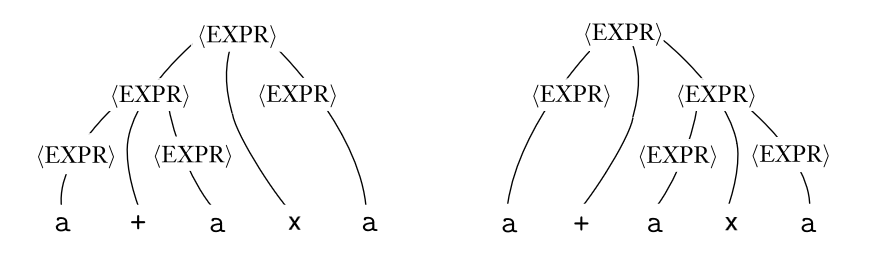
\includegraphics[scale=0.5]{img/ambiguita.png}\\
\end{center}
Questa due casi costituiscono un \g{ambiguità}.
\begin{itemize}
	\item Una stringa $w$ è derivata ambiguamente dalla grammatica $G$ se esistono due o più alberi sintattici che la generano
	\item \g{Equivalentemente}: Una stringa $w$ è derivata ambiguamente dalla grammatica $G$
		se esistono due o più derivazioni a sinistra che la generano
	\item Una grammatica è ambigua se genera almeno una stringa ambiguamente
\end{itemize}
\textit{Spesso dunque è preferibile ricavare una forma normalizzata di una CFG per poterla analizzare meglio.}\\
Una delle forme più semplici ed utili è appunto la forma normale di Chomsky. 

\subsubsection{Definizione della forma normale di Chomsky}
Una grammatica context-free è in forma normale di Chomsky se ogni regola è della forma 

$$A\rightarrow BC$$
$$A \rightarrow a$$Dove $a$ è un terminale e $B, C$ non possono essere la variabile iniziale. 
Inoltre, ci può essere la regola iniziale $S\rightarrow\varepsilon$ per la variabile iniziale $S$.

\begin{center}
	\textit{Ogni CFG è generata da una forma normale di Chomsky}\\
	di conseguenza\\
	\textit{Ogni CFG è riducibile ad una forma normale di Chomsky}
\end{center}

\subsubsection{Come passare ad una forma normale di Chomsky}
\begin{enumerate}
	\item aggiungiamo una nuova variabile iniziale
	\item eliminiamo le $\varepsilon$-regole $A \rightarrow\varepsilon$ 
	\item eliminiamo le regole unitarie $A\rightarrow B$ 
	\item trasformiamo le regole rimaste nella forma corretta
\end{enumerate}

\paragraph{Esempio}
Trasformiamo la grammatica $G_6$ in forma normale di Chomsky:
$$S\rightarrow ASA\mid aB$$
$$A\rightarrow B\mid S$$ $$B\rightarrow b\mid \varepsilon$$
\begin{enumerate}
	\item Aggiungiamo una nuova variabile iniziale $S_0\rightarrow S$ 
		\textit{Questo ci serve ad evitare che la variabile iniziale compaia a \g{destra} di una regola di derivazione}
	\item Eliminiamo le $\varepsilon$-regole $A\rightarrow\varepsilon$ 
		\begin{itemize}
			\item Se $A\rightarrow\varepsilon$ è una regola dove $A$ non è la variabile iniziale. 
			\item Per ogni regola del tipo $R\rightarrow uAv$ aggiungiamo la regola $$R\rightarrow uv$$
				\g{Attenzione}: Nel caso di più occorrenze di $A$ consideriamo tutti i casi: per le regole come 
			$R\rightarrow uvAw\mid uAvw\mid uvw$ 
			\item Nel caso di regole $R\rightarrow A$ aggiungiamo $R\rightarrow\varepsilon$ solo se non abbiamo già eliminato $R\rightarrow\varepsilon$ 
			\item ripetere fino a che non sono state eliminate tutte le $\varepsilon$-regole
		\end{itemize}

	\item  Eliminare le \g{regole unitarie} $A\rightarrow B$ :
		\begin{itemize}
			\item  Se $A\rightarrow B$ è una regola unitaria 
			\item Per ogni regola del tipo $B\rightarrow u$, aggiungiamo la regola unitaria eliminata in precedenza
			\item ripetere finché non sono state eliminate tutte le regole unitarie
		\end{itemize}
	\item Trasformiamo le regole rimaste nella forma corretta: 
		\begin{itemize}
			\item Se $A\rightarrow u_1u_2\dots u_k$ è una regola tale che 
				\begin{itemize}
					\item Ogni $u_i$ è una variabile o un terminale 
					\item $k\geq 3$ 
				\end{itemize}
			\item sostituisci la regola con la catena di regole 
	  		$A\rightarrow u_1A_1$, $A_1\rightarrow u_2A_2$, $A_@\rightarrow u_3A_3$ $\dots$ $A_{k-2}\rightarrow u_{k-1}u_k$ 
			\item  rimpiazza ogni terminale $u_i$; sul lato destro di una regola con una nuova variabile
				$U_i$ e aggiungi la regola $$U_i\rightarrow u_i$$
			\item ripetere per ogni regola non corretta
		\end{itemize}
\end{enumerate}
\newpage
\section{Automi a Pila}
Come preannunciato in [[Linguaggi Context-free]], gli automi a pila sono un metodo per definire alcuni \textit{linguaggi non regolari}.
Gli automi a pila (\textit{pushdown automata}, o \textit{PDA}) sono degli automi a cui viene affiancata una memoria detta 
\g{stack} (pila), e sono \g{computazionalmente equivalenti alle grammatiche context-free}. 
Un PDA può scrivere simboli nella pila e rileggerli in seguito. Scrivere un simbolo comporta "\textit{spingere giù}" i simboli della pila.
In qualsiasi momento il simbolo nella cima può essere letto e rimosso, esattamente come si comporta una memoria di tipo \textit{stack},
e dunque \g{LIFO} (last in first out).
Un automa a pila è composto da: 
\begin{itemize}
	\item \g{Input}: stringa di caratteri dell'alfabeto
	\item \g{Memoria}: stati + pila
	\item \g{Funzioni di transizione}: dato lo stato corrente, un simbolo di input ed il \textit{simbolo in cima alla pila},
		stabilisce quali possono essere gli stati successivi e i \textit{simboli da scrivere sulla pila}
\end{itemize}
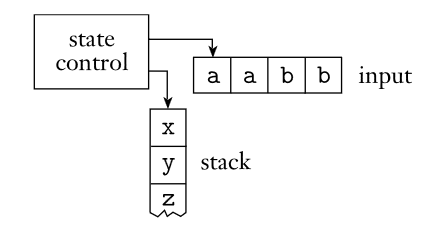
\includegraphics[scale=0.5]{img/schema_PDA.png}

Le operazioni di scrittura sono 
\begin{itemize}
	\item \g{push}: inserimento di un simbolo nella pila
	\item \g{pop}: lettura e rimozione di un simbolo dalla pila
\end{itemize}
Questo permette agli automi a pila di avere \textit{memoria infinita} \g{MA} \textit{con accesso limitato}.
Esempio: $\{0^n1^n | n \geq 0\}$

Un PDA usa la pila per contare 0 e 1:
\begin{itemize}
	\item legge i simboli in input, e *scrive* ogni 0 letto sulla pila
	\item non appena vede gli 1, *cancella* uno 0 dalla pila per ogni 1 letto
	\item se l’input termina esattamente quando la pila si svuota, **accetta**
	\item se ci sono ancora 0 nella pila al termine dell’input, *rifiuta*
	\item se la pila si svuota prima della fine dell’input, *rifiuta*
	\item se qualche 0 compare nell’input dopo gli 1, *rifiuta*
\end{itemize}


\begin{center}
	\Large\g{Attenzione}
\end{center}

Gli automi a pila possono essere \g{non deterministici}.
Automi a pila deterministici e non deterministici \textit{non} sono computazionalmente equivalenti, diversamente da quanto avviene tra DFA e NFA. 

\subsection{Definizione di PDA}
La definizione è simile a quella di un automa finito, tranne che per la pila. 
Tale pila *non utilizza necessariamente lo stesso linguaggio della stringa in input*
Per tanto un automa a pila è una sestupla $P=(Q,\Sigma,\Gamma,\delta, q_0, F)$:
\begin{itemize}
	\item $Q$ è l'insieme finito di \textit{stati}
	\item $\Sigma$ è l'alfabeto di \textit{input}
	\item $\Gamma$ è l'alfabeto della \textit{pila}
	\item $\delta:Q\times\Sigma_\varepsilon \times\Gamma_\varepsilon\mapsto 2^{Q\times\Gamma_\varepsilon}$ è la funzione di transizione
	\item $q_0\in Q$ è lo \textit{stato iniziale}
	\item $F\subseteq Q$ è l'insieme di \textit{stati accettanti} (dove $\Sigma_\varepsilon = \Sigma\cup\{\varepsilon\}$ e $\Gamma_\varepsilon = \Gamma\cup \{\varepsilon\}$)
\end{itemize}
\paragraph{Esempio}
\g{PDA per} $\{0^n1^n\mid n\geq 0\}$:\\
\begin{itemize}
\item $P = (\{q_0, q_1, q_2, q_3\}, \{0,1\}, \{0,\$\}, \delta,q_0,\{q_0,q_3\})$ 
\item con $\delta$ descritta dalla tabella:
	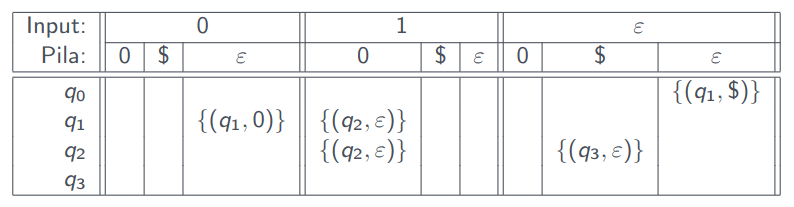
\includegraphics[scale=0.5]{img/tabella_delta.png}
	o dalla transizione
	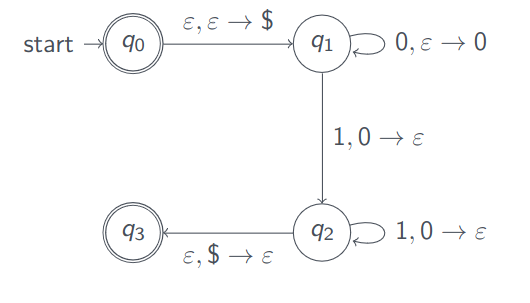
\includegraphics[scale=0.5]{img/transizione_delta.png}
\end{itemize}

\subsection{Computazione e linguaggi di un PDA}
Data una parola $w$, un PDA accetta la parola se:
\begin{itemize}
	\item possiamo scrivere $w = w_1w_2 \dots w_m$ dove $w_i \in \Sigma\cup \{\varepsilon\}$ 
	\item esistono una sequenza di stati $r_0, r_1,\dots, r_m \in Q$ e
	\item *una sequenza di stringhe* $s_0, s_1, s_2,\dots, s_m \in \Gamma^*$ 
\end{itemize}
\begin{center}
	tali che
\end{center}
\begin{enumerate}
	\item $r_0 = q_0$ e $s_0 = \varepsilon$ (inizia dallo stato iniziale e pila vuota)
	\item per ogni $i = 0, \dots, m - 1, (r_i+1, b) \in \delta(r_i , w_{i+1}, a)$ con $s_i = at$
		e $s_{i+1} = bt$ per qualche $a, b\in \Gamma_\varepsilon$ e $t\in\Gamma^*$ (l'automa rispetta la funzione
		di transizione)
	\item $r_m\in F$ (la computazione *termina in uno stato finale*)
\end{enumerate} 

\subsection{Accettazione per pila vuota}
La nostra definizione di PDA accetta le parole \textit{per stato finale}.
L'accettazione per pila vuota costituisce un altro un altro modo per definire la \textit{condizione di accettazione}:
Un PDA accetta la parola $w$ per pila vuota se esiste una computazione che
\begin{itemize}
	\item consuma tutto l’input
	\item termina con la pila vuota $(s_m = \varepsilon)$ 
\end{itemize}
\g{Equivalenza}\
\begin{theorem}
	Per ogni linguaggio accettato da un PDA per stato finale esiste un
	PDA che accetta per pila vuota, e viceversa
\end{theorem}

\begin{theorem}[Equivalenza con le grammatiche context-free]
	Un linguaggio è context-free se e solo se esiste un PDA che lo riconosce.
\end{theorem}
Sappiamo che un linguaggio è context-free se esiste una CFG che lo genera 
Mostreremo come trasformare la grammatica in un PDA e, viceversa, come trasformare un PDA in una grammatica. 

\begin{lemma}
	Se un linguaggio è context-free, allora esiste un PDA che lo riconosce
\end{lemma}
Per fare convertire una CFG in PDA è importante tenere a mente che ogni passo di derivazione produce una **stringa intermedia** contenente variabili e terminali.
Data una stringa $w$ il PDA dev'essere progettato in modo da stabilire se una serie di sostituzioni effettuate secondo le regole della CFG possa condurre dalla variabile iniziale a $w$.
Per fare questo è fondamentale sfruttare il **non determinismo** del PDA per poter effettuare le sostituzioni che portano a $w$. 
Il PDA inizia scrivendo la variabile iniziale sulla pila. 

\g{Idea}:
\begin{itemize}
	\item Se $L$ è context-free, allora esiste una CFG $G$ che lo genera
	\item Mostriamo come trasformare $G$ in un PDA equivalente $P$
	\item $P$ è fatto in modo da *simulare* i *passi di derivazione* di $G$
	\item $P$ accetta $w$ se esiste una derivazione di $w$ in $G$
\end{itemize}

\subsubsection{Rappresentare le stringhe intermedie}
\begin{itemize}
	\item La **pila** memorizza le stringhe intermedie
	\item $P$ trova le variabili nella stringa intermedia e fa le sostituzioni
  	seguendo le regole di $G$ 
	\item **Idea**: metto nella pila solo **i simboli dalla prima variabile in poi**
		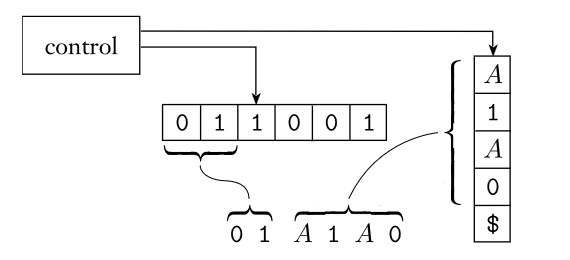
\includegraphics[scale=0.5]{img/stringhe_intermedie.png}
	\item Ogni derivazione è una sequenza di **stringhe intermedie**
\end{itemize}

$S\rightarrow 0S1\mid\varepsilon$ 
$S\Rightarrow 0S1\Rightarrow 00S11\Rightarrow 0011$
L'automa partirà dalla variabile iniziale, poi supponiamo che l'automa si trovi in $00S11$ 
Grazie alle transizioni elaborate avremo la pila 

0
0
S  In questo caso l'automa trova una variabile e applica una regola $(0S1\mid\varepsilon)$
1
1
\$  Ad indicare la fine della pila 

\subsection{Definizione informale del PDA}
\begin{enumerate}
	\item Inserisci il simbolo marcatore $\$$ e la variabile iniziale $S$  sulla pila
	\item  Ripeti i seguenti passi:
		\begin{enumerate}
			\item Se la cima della pila è la variabile $A$: scegli una regola $A\rightarrow u$ e 
				scrivi $u$ sulla pila (qui si sfrutta il non determinismo )
			\item Se la cima della pila è un terminale $a$: leggi il prossimo simbolo
				di input.
				\begin{itemize}
					\item se sono uguali, procedi
					\item se sono diversi, rifiuta
				\end{itemize}
		\end{enumerate}
	\item Se la cima della pila è $\$$: vai nello stato accettante
\end{enumerate}

\subsection{Notazione compatta}
Supponiamo che il PDA vada da $q$ z $r$ quando legge $a$ e fa il pop di $s$ 
... inserendo la **stringa** di tre caratteri $u=xyz$ sulla pila, per farlo sono necessarie 3 transizioni come nell'immagine 
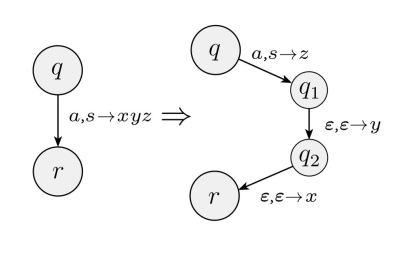
\includegraphics[scale=0.5]{img/notazione_compatta.png}

Per implementare il push multiplo dobbiamo **aggiungere stati ausiliari**  

\subsection{Dimostrazione}
Data $G=(V,\Sigma, R, S)$ definiamo $P=(Q,\Sigma,\Gamma,q_{start},F)$ 
\begin{itemize}
	\item $Q=\{q_{start}, q_{loop}, q_{end}\}$ 
	\item $\Gamma = \Sigma \cup V \cup \{\$\}$ 
	\item $F=\{q_{end}\}$ 
	\item funzione di transizione
\end{itemize}
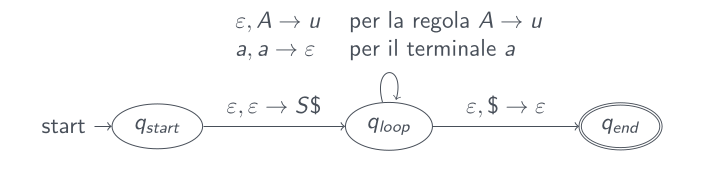
\includegraphics[scale=0.5]{img/dimostrazione_pda.png}

\subsection{Da PDA a grammatica Context-Free}
Abbiamo un PDA $P$ che riconosce il linguaggio 
Mostriamo come trasformare $P$ in una CFG equivalente $G$ 
\begin{itemize}
	\item Una stringa $w$ accetta da $P$ se fa andare $P$ dallo stato iniziale a quello finale
	\item Progetteremo una grammatica che **fa un po' di più** 
		\begin{itemize}
			\item Una variabile $A_{pq}$ per ogni coppia di stati $p,q$ di $P$ 
			\item $A_{pq}$ genera tutte le stringhe che portano **da** $p$ **con pila vuota** a $q$ **con pila vuota**
		\end{itemize}
\end{itemize}
Come prima cosa, semplifichiamo $P$ in modo che rispetti tre condizioni:
\begin{enumerate}
	\item ha un unico stato accettante $q_f$ 
	\item svuotiamo la pila prima di accettare
	\item  Ogni transizione **inserisce un unico simbolo sulla pila (push)** oppure **elimina un simbolo dalla pila (pop)**, ma non fa entrambe le cose contemporaneamente. 
\end{enumerate}

\paragraph{Andare da $P$ a $q(1)$}
Per andare da $p$ con pila vuota a $q$ con pila vuota:
\begin{itemize}
	\item la prima mossa deve essere necessariamente un push 
	\item l'ultima mossa deve essere un pop
\end{itemize}
Ci sono due casi:
\begin{enumerate}
	\item Il simbolo inserito all'inizio viene eliminato alla fine:
		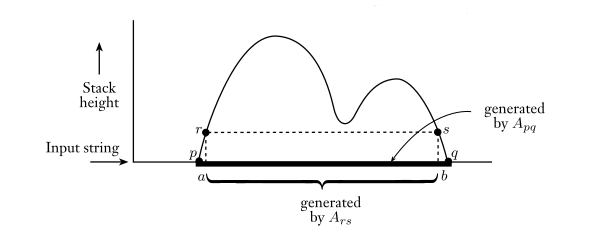
\includegraphics[scale=0.5]{img/da_p_a_q.png}
		Per ogni coppia di transizioni che effettuano il push e il pop di un determinato simbolo andremo ad aggiungere una regola:
		$A_{pq}\rightarrow aA_{rs}b$ 
	\item Oppure no, il simbolo inserito all'inizio viene rimosso prima di terminare la computazione.
		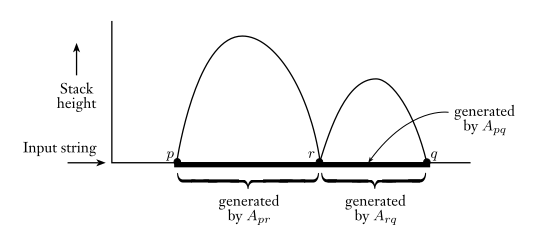
\includegraphics[scale=0.5]{img/da_p_a_q_2.png}
		in questo caso dobbiamo aggiungere la regola
		$\forall p,q,r\in Q$ 
		$A_{pq}\rightarrow A_{pr}A_{rq}$
		$A_{pq} \rightarrow\varepsilon$ per ogni $q\in Q$ 
\end{enumerate}

\paragraph{Le regole di $G$}
Formalmente 
\begin{itemize}
	\item sia $P=(Q,\Sigma,\Gamma, \delta, q_0,\{q_r\})$ 
	\item costruiamo $G=(V\Sigma, R, A_{q0}, q_r)$ tale che 
		\begin{itemize}
			\item $V =\{A_{pq}, p, q\in Q \}$
			\item Per ogni $p,q,r,s,\in Q$, $u\in\Gamma$ e $a,b\in\Sigma$, se $\delta(p,a,\varepsilon)$ contiene $(r,u)$ e $\delta(s,b,u)$ contiene $(q,\varepsilon$ ), aggiungi la regola $A_{pq}\rightarrow aA_{rs}b$ 
			\item Per ogni $p,q,r,\in Q$, aggiungi la regola $A_{pq}\rightarrow A_{pr}A_{rq}$ 
			\item Per ogni $p\in Q$, aggiungi la regola $A_{pp}\rightarrow \varepsilon$ 
		\end{itemize}
\end{itemize}

\paragraph{Due dimostrazioni induttive}
\paragraph{Lemma}
Se $A_{pq}$ genera la stringa $x$, allora $x$ può portare $P$ da $p$ con pila vuota a $q$ con pila vuota
\paragraph{Lemma}
Se la stringa $x$ può portare $P$ da $p$ con pila vuota a $q$ con pila vuota, allora $A_{pq}$ genera $x$. 

\begin{theorem}
	Un linguaggio è context-free se e solo se esiste un PDA che lo rionosce 
\end{theorem}
\begin{itemize}
	\item Sappiamo che un linguaggio è context-free se esiste una CFG che lo genera
	\item Abbiamo mostrato come trasformare una CFG in un PDA
	\item E viceversa, come trasformare un PDA in grammatica
\end{itemize}



\newpage
\section{Macchine di Turing}
\subsection{La Tesi di Church-Turing}
Finora abbiamo visto DFA con una quantità finita di memoria. I PDA che hanno memoria illimitata ma ad accesso limitato (abbiamo solo operazioni *push* e *pop*).
Questo comporta dei limiti alla loro capacità di computazione. 

\subsection{Macchina di Turing}
È un modello proposto da Alan Turing nel 1936 per risolvere problemi matematici.
\begin{itemize}
	\item Ha memoria illimitata, utilizza un nastro infinitoj/
	\item Non ci sono restrizioni di accesso alla memoria
\end{itemize}
Una macchina di Turing è un modello molto più preciso di un computer. 

\g{Tuttavia...}
\begin{itemize}
	\item Ci sono problemi che una Macchina di Turing **non può risolvere**
	\item questi problemi *vanno oltre le capacità di un computer*
\end{itemize}
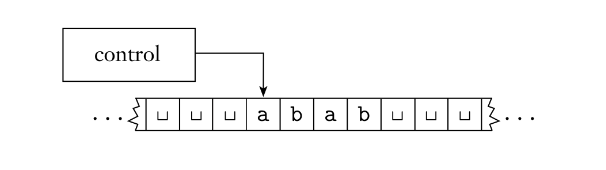
\includegraphics[scale=0.5]{img/schema_TM.png}

la macchina di Turing è composte da 
\begin{itemize}
	\item un nastro infinito come **memoria illimitata**
	\item una testina che **legge e scrive** simboli sul nastro
	\item all'inizio il nastro contiene l'input
	\item per memorizzare informazione si **scrive sul nastro** 
	\item la testina si può muovere **ovunque sul nastro**
	\item stati speciali per \g{accetta} e \g{rifiuta} 
\end{itemize}

\subsection{Primo esempio di TM}
Costruiamo una macchina di Turing per il linguaggio 
$$ B = \Big\{ w\# w \mid w\in \{0,1\}^* \Big\}$$
\begin{itemize}
	\item $M_1$deve accettare se l'input sta in $B$, e rifiutare altrimenti
	\item $M_1$= ''su input $w$:
\end{itemize}
\begin{enumerate}
	\item Si muove a zig-zag lungo il nastro, raggiungendo posizioni corrispondenti ai due lati di $\#$ per controllare se contengono lo stesso simbolo. In caso negativo, o se non trovi $\#$, \g{rifiuta}.
		Barra gli elementi già controllati 
	\item Se tutti i simboli a sinistra di $\#$ sono stati controllati, verifica i simboli a destra di $\#$. Se c'è qualche simbolo ancora da controllare \g{rifiuta}, altrimenti \g{accetta} 
\end{enumerate}
Questa descrizione della macchina di Turing $M_1$ ne illustra il funzionamento ma non ne mostra tutti i dettagli. 

\subsection{Automi finiti vs Macchine di Turing}
\begin{enumerate}
	\item Una TM può sia scrivere che leggere sul nastro
	\item  Una TM può muoversi si a a destra che a sinistra
	\item  Il nastro è infinito
	\item  Gli stati di rifiuto e accettazione hanno effetto immediato
\end{enumerate}

\subsection{Definizione formale}
Una macchina di Turing è una tupla $M = \{Q, \Sigma, \Gamma,\delta, q_0, q_{accept},q_{reject}\}$ 
	\begin{itemize}
	\item $Q$ è l'insieme finito di **stati**
	\item $\Sigma$ è l'**alfabeto di input** che non contiene il simbolo **blank**
	\item $\Gamma$ è l'**alfabeto del nastro** che contiene $\textvisiblespace$ e $\Sigma$ 
	\item $\delta : Q\times \Gamma\rightarrow Q\times\Gamma\times\{L,R\}$ è la **funzione di transizione** 
	\item $q_0\in Q$ è lo  **stato iniziale** 
	\item $q_{accept}\in Q$ è lo **stato di accettazione**
	\item $q_{reject}\in Q$ è lo **stato di rifiuto** (necessariamente diverso da $q_{accept}$ )
\end{itemize}
Nella macchina di Turing la funzione di transizione è la parte fondamentale. 

\subsection{Configurazioni}
Lo stato corrente, la posizione della testina e il contenuto del nastro formano a **configurazione** di una TM.
Dalla configurazione possiamo sapere la \g{prossima mossa}
Le configurazioni sono rappresentate da una tripla $uqv$:
\begin{itemize}
	\item $q$ è lo **stato corrente**
	\item $u$ è il contenuto del **nastro prima della testina** 
	\item $v$ è il contenuto del **nastro dalla testina in poi** 
	\item la testina si trova **sul primo simbolo di** $v$ 
\end{itemize}

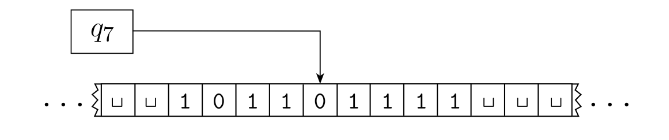
\includegraphics[scale=0.5]{img/tm_conf.png}
(la configurazione in figura è $1011q_701111$)

\subsection{Computazione}
La configurazione $C_1$ \b{produce} $C_1$ se la TM può passare da $C_1$ a $C_2$ in un passo
Se $a,b,c\in\Gamma$, $u,v\in\Gamma^*$ e $q_i, q_j$ sono stati, allora
	$uaq_ibv$ produce $uq_jacv$ se $\delta(q_i, b)= (q_i, c, L)$ 
	$uaq_ibv$ produce $uacq_jv$ se $\delta(q_i, b)= (q_i, c, R)$ 
\begin{itemize}
	\item la \g{configurazione iniziale} con input $w$ è $q_0w$ 
	\item in una \g{configurazione di accettazione} lo stato è $q_{accept}$ 
	\item in una \g{configurazione di rifiuto} lo stato è $q_{reject}$
\end{itemize}
\subsection{Linguaggi Turing-riconoscibili}
Una TM $M$ \g{accetta} l'input $w$ se esiste una **sequenza di configurazioni** $C_1, C_2,\dots, C_k$ tale che: 
\begin{itemize}
	\item $C_1$ è la configurazione iniziale con input $w$ 
	\item Ogni $C_i$ produce $C_{i+1}$ 
	\item $C_k$ è una configurazione di accettazione
\end{itemize}
Il \g{Linguaggio riconosciuto da} \textit{M} è l'insieme delle stringhe accettate da $M$ 

\begin{theorem}
	Un linguaggio è <i>Turing-riconoscibile</i> (o anche <i>ricorsivamente enumerabile</i>) se esiste una macchina di Turing che lo riconosce
\end{theorem}
</center>

\subsection{Linguaggi Turing-decidibili}
Se forniamo un input ad una TM, ci sono \g{tre risultati possibili}:
\begin{itemize}
	\item la macchina \g{accetta}
	\item la macchina \g{rifiuta} 
	\item la macchina va in \g{loop} e non si ferma mai
\end{itemize}
La TM può non accettare sia rifiutando che andando in loop.
Un TM che termina sempre la computazione è un \g{decisore} 
Un decisore \g{decide} un linguaggio se lo riconosce 

\begin{theorem}
	Un linguaggio è <i>Turing-decidibile</i> (o anche <i>ricorsivo</i>) se esiste una macchina di Turing che lo decide
\end{theorem}

\subsection{Esempi}
\subsubsection{Esempio 1}
TM che \g{decide} il linguaggio di tutte le stringhe di $0$ la cui lunghezza è una potenza di 2:
$$A = \{0^{2^n}\mid n\geq 0\}$$
$M_1=$ "su input $w$: 
\begin{enumerate}
	\item Scorri il nastro da sinistra a destra, cancellando ogni secondo $0$ 
	\item Se il nastro conteneva un solo $0$, \g{accetta}
	\item Se il nastro conteneva un numero dispari di $0$, \textit{rifiuta}
	\item  Ritorna all'inizio del nastro
	\item  Vai al passo 1"
\end{enumerate}

\subsubsection{Esempio 2}
% link primo esempio di TM
vedi Primo esempio di TM

\subsubsection{Esempio 3}
TM che esegue operazioni aritmetiche.  Decide il linguaggio
$C=\{a^ib^jc^k\mid k = i\cdot j$ e $i,j,k\geq 1\}$ 

$M_3=$ "su input $w$:
\begin{enumerate}
	\item Scorri il nastro da sinistra a destra e controlla se l'input sta in $a^+b^+c^+$. \g{rifiuta} se non lo è
	\item Ritorna all'inizio del nastro
	\item Barra una $a$ e scorri a destra fino a trovare una $b$. Fai la spola tra $b$ e $c$, barrando le $b$ e le $c$ fino alla fine delle $b$. Se tutte le $c$ sono barrate e rimangono ancora $b$, \textit{rifiuta}.
	\item Ripristina le $b$ barrate e ripeti \item finché ci sono $a$ da barrare.
	\item Quando tutte le $a$ sono barate, controlla se tutte le $c$ sono barrate: se sì, \g{accetta}; altrimenti \textit{rifiuta}."
\end{enumerate}

\subsubsection{Esempio 4}
TM che risolve il problem degli **elementi distinti**. Prende in input una sequenza di stringhe separate da $\#$ e accetta se tutte le stringhe sono diverse. 
Decide il linguaggio:
$D=\{\#x_1\#x_2\#\dots\#x_l\mid x_j\in \{0,1\}^*$ e $x_i\neq x_j$ per ogni $i\neq j\}$ 

$M_4=$ "su input $w$ 
\begin{enumerate}
	\item Mette un segno sul simbolo del nastro più a sinistra. Se è un blank, \g{accetta}. Se è un $\#$, continua con \item Altrimenti, \textit{rifiuta}.
	\item Scorre a destra fino al successivo $\#$ e vi mette sopra un secondo segno. Se nessun $\#$ viene trovato, allora era presente solo $x_1:$ \g{accetta}.
	\item Procede a zig-zag confrontando le due stringhe a destra dei $\#$ segnati. Se sono uguali, \g{rifiuta}
	\item Sposta il segno più a destra sul successivo $\#$ alla sua destra.Se non trova nessun $\#$, sposta il segno più a sinistra sul successivo $\#$ alla sua destra, e sposta il segno più a destra sul successivo $\#$. Se on c'è un $\#$ dopo il segno più a destra, allora tutte le stringhe sono state confrontate: \g{accetta}
	\item Vai alla fase 3.
\end{enumerate}

\subsection{Conclusioni}
\begin{itemize}
	\item I linguaggi $A, B, C$ e $D$ sono \textit{decidibili}
	\item Tutti i linguaggi Turing-decidibili sono anche Turing-riconoscibili
	\item I linguaggi $A,B,C$ e $D$ sono anche \textit{Turing-riconoscibili}
	\item Vedremo che ci sono linguaggi \textit{Turing-riconoscibili ma non decidibili}
\end{itemize}

\newpage
\section{Varianti di Macchine di Turing}
Esistono definizioni alternative delle macchine di Turing, chiamiamo \g{varianti}  queste alternative.
Tutte le varianti ``ragionevoli'' riconoscono \textit{la stessa classe di linguaggi}
Le Turing machine sono un modello \textit{robusto}.

\subsection{Macchine a nastro semi-infinito}

\begin{itemize}
   \item È una Turing Machine con un nastro \textit{infinito solo verso destra}.
   \item L'input si trova \textit{all'inizio del nastro}
   \item La testina parte dalla \textit{posizione più a sinistra del nastro}
   \item Se \textit{M} tenta di spostare la testina a sinistra quando si trova nella prima cella del nastro, allora \textit{la testina rimane ferma}.
\end{itemize}
\begin{theorem}
   \item Per ogni TM a nastro semi-infinito \textit{esiste} una TM a nastro infinito equivalente
   \item Per ogni TM a nastri infinito \textit{esiste} una TM a nastro semi-infinito equivalente
\end{theorem}

\subsection{Macchine Multinastro}
È una TM con $k$ nastri semi-infiniti, $k$ testine di lettura e scrittura, l'input si trova sul nastro 1.
Ad ogni passo scrive e si muove simultaneamente su tutti i nastri. 
Funzioni di transizione: 
$$\delta:Q\times\Gamma^k\rightarrow Q\times\Gamma^k\times\{L, R\}^k$$
$$\delta(q_i, a_1,\dots, a_k)=(q_j, b_1, \dots, b_k,L,R,\dots, L)$$
se lo stato è $q_i$ e le testine leggono $a_1, \dots, a_k$ allora scrivi $b_1,\dots, b_k$ sui $k$ nastri.
Muovi ogni testina a sinistra o a destra come specificato.

\begin{theorem}{Equivalenza}
   Per ogni TM multinastro esiste una TM a singolo nastro equivalente
\end{theorem}
{\Large FOTO}
$S=$ "Su input $w = w_1\dots w_n$ :
\begin{enumerate}
   \item Inizializza il nastro per rappresentare i $k$ nastri:
      $$\#w_1w_2\dots w_n\#\textvisiblespace\#\textvisiblespace\#\dots\#$$
   \item  Per simulare una mossa di $M$, scorri il nastro per determinare i simboli puntati dalle testine virtuali
   \item  Fai un secondo passaggio del nastro per aggiornare i nastri virtuali secondo la funzione di transizione di $M$ 
   \item  Se $S$ sposta una testina virtuale a destra su un $\#$, allora $M$ ha spostato la testina sulla parte vuota del nastro. 
      Scrivi un $\textvisiblespace$ e sposta il contenuto del nastro di una cella a destra. 
   \item  Se si raggiunge una configurazione di accettazione, \g{accetta}*, se si raggiunge una configurazione di rifiuto, \textit{rifiuta},
      altrimenti ripeti da 2.
\end{enumerate}

\begin{corollary}
   Un linguaggio è \textit{Turing-riconoscibile} \g{se e solo se} esiste una macchina di Turing \textit{multinastro} che lo riconosce. 
   $\Rightarrow$ \\
   Un linguaggio è Turing-riconoscibile se è riconosciuto da una TM con un nastro, che è un caso particolare di TM multinastro. 
   $\Leftarrow$ \\
   Costruzione precedente 
\end{corollary}

\subsection{Macchine non deterministiche}
Una TM non deterministica ha \g{più strade possibili} durante la computazione. 
Consideriamo macchine con un solo nastro semi-infinito.
La funzione di transizione è:
$$\delta:Q\times\Gamma\rightarrow 2^{(Q\times\Gamma\times\{L,R\})}$$
La computazione è un \g{albero} che descrive le scelte possibili.
La macchina accetta se \g{esiste un ramo} che porta allo stato di accettazione\\
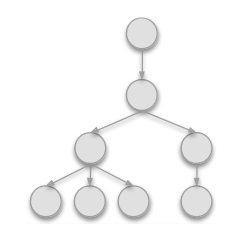
\includegraphics[scale=0.5]{img/albero.png}\\
\g{Tutti i rami} devono essere esaminati fino a quando non viene trovato uno \g{stato di accettazione}.
Come esaminare l'albero:
\textit{in ampiezza} o \textit{in profondità}?

\begin{theorem}
   Per ogni TM \g{non deterministica} esiste una TM \g{deterministica} equivalente
\end{theorem}
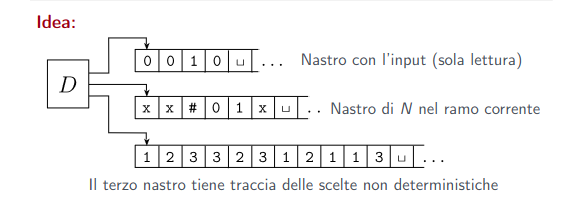
\includegraphics[scale=0.8]{img/idea_non_deterministica.png}

\subsection{Come funziona il terzo nastro }
Ad ogni nodo viene assegnato un \g{indirizzo}: una stringa sull'alfabeto $\Gamma_b = \{1,2,\dots,b\}$, 
dove $b$ è il massimo numero di figli dei nodi dell'albero: \\
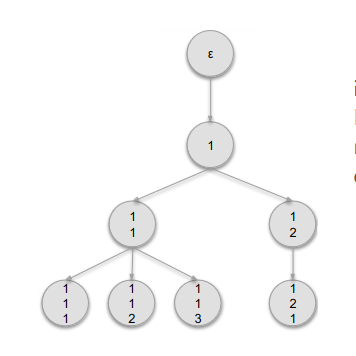
\includegraphics[scale=0.5]{img/albero_2.png}\\
Il nodo 113 si raggiunge prendendo il \g{primo} figlio della radice, seguito dal \g{primo} figlio di quel modo ed infine dal \g{terzo} figlio. 
Questo ordinamento può essere utilizzato per attraversare in modo efficiente l'albero in ampiezza.\\
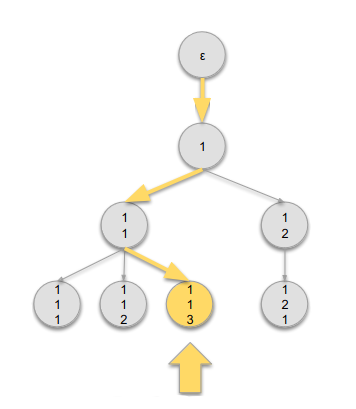
\includegraphics[scale=0.5]{img/albero_3.png}

\subsection{Come funziona $D$}
\begin{enumerate}
   \item Inizialmente il nastro 1 contiene l'input $w$ e i nastri 2 e 3 sono vuoti. 
   \item Copia il nastro 1 sul nastro 2 e inizializza la stringa sul nastro 3 a $\varepsilon$ 
   \item Usa il nastro 2 per simulare $N$ con input $w$ su un ramo di computazione.
      Prima di ogni passo di $N$, consulta il simbolo successivo sul nastro 3 per determinare quale scelta fare (tra quelle consentite).
      Se non rimangono più simboli sul nastro 3, o se questa scelta non è valida, interrompi questo ramo e vai alla fase 4. 
      Vai ala fase 4. anche se si incontra una configurazione di rifiuto.
      Se viene trovata una configurazione di accettazione, \g{accetta}.
   \item Sostituire la stringa sul nastro 3 con la stringa successiva nell'ordine delle stringhe. Simula il ramo successivo di $N$ andando alla fase 2. 
\end{enumerate}

\subsection{Conclusione}
\begin{corollary}
   Un linguaggio è Turing-riconoscibile se e solo se esiste una macchina di Turing \g{non deterministica} che lo riconosce.\\
   $\Rightarrow$ Un linguaggio è Turing-riconoscibile se è riconosciuto da una TM deterministica, che è un caso particolare di TM non deterministica. \\
   $\Leftarrow$ Costruzione precedente 
\end{corollary}

\subsection{Enumeratori}
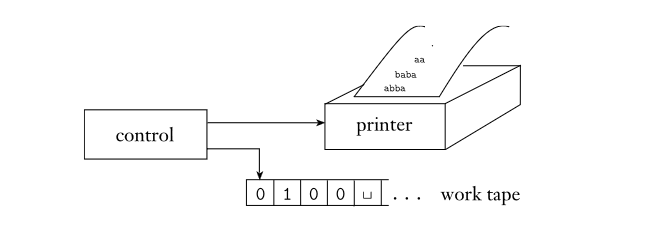
\includegraphics[scale=0.5]{img/enumeratore.png}\\
L'enumeratore è una macchina di Turing che dispone di una stampante.
\begin{itemize}
   \item Un emumeratore $E$ inizia con \g{nastro vuoto}.
   \item Di tanto in tanto, \g{invia una stringa alla stampante} 
   \item Linguaggio \g{enumerato} da $E:$ tutte le stringhe stampate
   \item $E$ può generare le stringhe in qualsiasi ordine, anche con ripetizioni. 
\end{itemize}

\subsection{Equivalenza}
\begin{theorem}
   Un linguaggio è Turing-riconoscibile se e solo se esiste un enumeratore che lo enumera
\end{theorem}
\g{Idea}: dobbiamo mostrare che 
\begin{itemize}
   \item se esiste un enumeratore $E$, allora esiste una TM $M$ che riconosce lo stesso linguaggio 
   \item se esiste una TM $M$ che riconosce il linguaggio, allora possiamo costruire un enumeratore
\end{itemize}

\subsection{Macchine di Turing monodirezionali}
\begin{itemize}
   \item Una macchina di Turing con ``resta ferma'' invece di ``muovi a sinistra''
   \item Funzione di transizione: $\delta : Q\times\Gamma\rightarrow Q\times\Gamma\{S,R\}$ 
   \item Ad ogni passo, la TM può lasciare ferma la testina o muoverla a destra
   \item \textit{Non può muoversi a sinistra}
\end{itemize}

\g{Quale classe di linguaggi riconosce?}

\subsection{Equivalenza con altri modelli}
\begin{itemize}
   \item Esistono altri modelli di computazione universali
   \item Alcuni sono molto simili alle macchine di Turing
   \item Altri sono molto diversi 
   \item Hanno tutti una caratteristica comune:
      \g{accesso senza restrizioni} ad una \g{memoria illimitata} 
   \item Sono \g{tutti equivalenti tra loro} 
\end{itemize}
\newpage
\section{Varianti di Macchine di Turing}
\g{Contesto storico}\\
David Hilbert, discorso al Secondo Congresso Internazionale di Matematica, Parigi, 1900
\begin{itemize}
	\item Definisce 23 problemi matematici come sfida per il nuovo secolo 
	\item \g{Decimo problema}: creare un algoritmo per determinare se un polinomio ha una radice intera
	\item Il presupposto era che \g{l'algoritmo dovesse esistere}, e bastava trovarlo
	\item Ora sappiamo che questo problema è \g{non risolvibile algoritmicamente} 
\end{itemize}

\subsection{Cos'è un algoritmo}
La \g{nozione intuitiva} di algoritmo esiste da migliaia di anni, mentre la \g{definizione formale}
di algoritmo è stata data per la prima volta nel XX secolo. 
Senza una definizione formale, è quasi \g{impossibile provare} che un algoritmo non può esistere. 

\subsubsection{Tesi di Church-Turing}
\begin{description}
	\item[1936] Church pubblica un formalismo chiamato
		$\lambda$-calcolo per definire algoritmi. 
	\item[1936] Turing pubblica le specifiche per una 
		\textit{macchina astratta} per definire algoritmi
	\item[1952] Kleene mostra che i due modelli sono 
		\g{equivalenti} 
	\item[1970] Matiyasevich dimostra che l'algoritmo per 
		stabilire se un polinomio ha radici intere **non esiste**
\end{description}

\subsubsection{Il decimo problema di Hilbert }
Il decimo teorema di Hilbert con la nostra terminologia 
$D=\{p\mid p$ è un polinomio avente radice intera$\}$ 
\begin{itemize}
	\item Il problema diventa \g{``$D$ è un insieme decidibile?''}
	\item Possiamo mostrare che $D$ è \g{Turing-riconoscibile} 
	\item Partiamo da un problema più semplice 
\end{itemize}
$D_1=\{p\mid p$ è un polinomio su $x$ avente radice intera$\}$ 

\subsection{Come descrivere una Turing Machine}
\begin{itemize}
	\item Descrizione formale
		\begin{itemize}
			\item Dichiara esplicitamente tutto quanto
			\item Estremamente dettagliata
			\item Da evitare a tutti i costi!!!
		\end{itemize}
	\item Descrizione implementativa
		\begin{itemize}
			\item Descrive a parole il movimento della testina e la scrittura sul nastro
			\item Nessun dettaglio sugli stati 
		\end{itemize}
	\item  Descrizione di alto livello
		\begin{itemize}
			\item Descrizione a parole dell'algoritmo
			\item Nessun dettaglio implementativo 
			\item Da utilizzare sempre, se non indicato altrimenti
		\end{itemize}
\end{itemize}

\subsubsection{Notazione formale per macchine di Turing}
\begin{itemize}
	\item L'input è sempre una \g{stringa} 
	\item Se l'input e un oggetto, deve essere rappresentato come una stringa
		\begin{itemize}
			\item  Polinomi, grammatiche, automi, ecc$\dots$ 
			\item L'input può essere una combinazione di diversi tipi di oggetti.
		\end{itemize}
	\item Un oggetto $O$ codificato come stringa è $\langle O\rangle$ .
	\item Una sequenza di oggetti $O_1, O_2,\dots, O_k$ è codificata come $\langle O_1, O_2,\dots, O_k\rangle$ 
	\item L'algoritmo viene descritto con un \g{testo}, indentato e con struttura a blocchi. 
	\item La prima riga dell'algoritmo descrive l'**input** macchina
\end{itemize}

\paragraph{Esempio: un problema di grafi}
I grafi sono strutture dati che vengono usate estensivamente in informatica.\\
Ci sono migliaia di problemi computazionali che sono importanti per le applicazioni e che si possono modellare con i grafi.\\
Vedremo ora che cos'è un grafo, e studieremo alcuni problemi sui grafi che sono interessanti per la loro \g{classe di complessità}.

\paragraph{Definizione di base}
Un grafo \g{non orientato} (detto anche \g{indiretto}) $G$ è una coppia $(V,E)$ dove
\begin{itemize}
	\item $V = \{v_1, v_2,\dots,v_n\}$ è un insieme finito e non un vuoto di vertici
	\item $E\subseteq \Big\{\{u,v\}\mid u,v\in v\Big\}$ è un insieme di \g{coppie non ordinate},
		ognuna delle quali corrisponde ad un **arco non orientato** del grafo. 
\end{itemize}
\paragraph{Definizione}
	Un grafo è \g{connesso} se ogni nodo può essre raggiunto da ogni altro nodo tramite gli archi del grafo. 

\paragraph{Problema }
Il linguaggio $A=\{\langle G\rangle\mid G$ è un grafo connesso $\}$ è decidibile? 

Definiamo una Turing Machine che decide $A$ 

\paragraph{Descrizione di alto livello}\nin\\
$M =$ "Su input $\langle G\rangle$, la codifica di un grafo $G$: 
\begin{enumerate}
	\item \g{Seleziona} il primo nodo $G$ e lo marca.
	\item  \g{Rpeti} la fase seguente fino a quando non vengono marcati nuovi nodi: 
	\item  Per ogni nodo in $G$, \g{marcalo} se è connesso con un arco ad un nodo già marcato
	\item  \g{Esamina} tutti i nodi di $G$:  se sono tutti marcati, \g{accetta}, altrimenti \textit{rifiuta}
\end{enumerate}

\paragraph{Codifica del grafo }
Codifica di $G$: lista dei nodi $+$ lista degli archi 
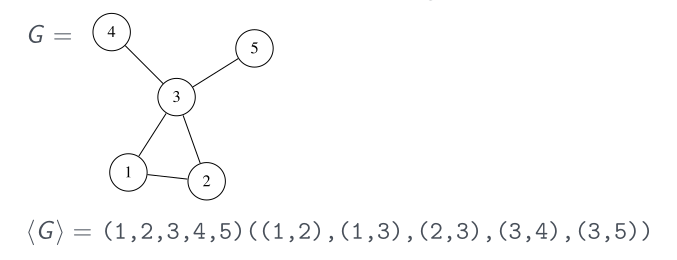
\includegraphics[scale=0.5]{img/codifica_grafo.png}
$M$ verifica che l'input \g{sia una codifica di un grafo}
\begin{itemize}
	\item Se l'input non è nella forma corretta, \g{rifiuta} 
	\item Se l'input codifica un grafo, prosegue con la fase 1
\end{itemize}
\newpage
\section{Linguaggi decidibili}
Obiettivi
\begin{itemize}
	\item Studiare il potere degli algoritmi
	\item Capire quali problemi sono risolvibili da un algoritmo e quali no
	\item In questa lezione iniziamo considerando problemi **decidibili** 
\end{itemize}

\subsection{Problemi sui linguaggi regolari}
\subsubsection{Problema dell'accettazione}
Ovvero, testare se un DFA accetta una stringa
$A_{DFA} = \{\langle B,w\rangle\mid B$  è un DFA che accetta la stringa $w\}$ 
$B$ accetta $w$ **se e solo se** $\langle B,w\rangle$ appartiene ad $A_{DFA}$ 
Mostrare che il linguaggio è **decidibile** equivale a mostrare che il problema computazionale è**decidibile**. 

\begin{theorem}{$A_{DFA}$ è decidibile}\end{theorem}
\g{Idea}: definire una TM che decide $A_{DFA}$ 
$M=$ "Su input $\langle B,w\rangle$, dove $B$ è un DFA e $w$ una stringa: 
\begin{enumerate}
	\item Simula $B$ su input $w$ 
	\item Se la simulazione termina in uno stato finale, \g{accetta}. Se termina in uno stato non finale, \textit{rifiuta}."
\end{enumerate}
	

\paragraph{Dimostrazione}
\begin{itemize}
	\item la codifica di $B$ è una lista dei componenti: $Q,\Sigma,\delta, q_0$ e $F$ 
	\item fare la simulazione è facile
\end{itemize}


\begin{theorem}{$A_{NFA}$ è decidibile}\end{theorem}
$A_{NFA} = \{\langle B,w\rangle\mid B$ è un $\varepsilon$-NFA che accetta la strina $w\}$ 
\g{Idea}: usiamo la TM $M$ che decide $A_{DFA}$ come subroutine.

\g{Dimostrazione}: 
$N=$ ``Su input $\langle B,w\rangle$, dove $B$ è un $\varepsilon$-NFA e $w$ una stringa: 
\begin{enumerate}
	\item Trasforma $B$ in un DFA equivalente $C$ usando la costruzione per sottoinsiemi
	\item Esegui $M$ con input $\langle C,w\rangle$ 
	\item  Se $M$ accetta, \g{accetta}; altrimenti, \textit{rifiuta}.''
\end{enumerate}
$N$ è un decisore per $A_{NFA}$, quindi $A_{NFA}$ è **decidibile**. 

\begin{theorem}$A_{REX}$ è decidibile\end{theorem}
$A_{REX} = \{\langle R, w\rangle\mid R$ è una espressione regolare che genera la stringa $w$ $\}$ 
\g{Idea}: usiamo la TM $N$ che decide $A_{NFA}$ come subroutine

\b{Dimostrazione}:
$P=$ ``Su input $\langle R,w\rangle$, dove $R$ è una espressione regolare e $w$ una stringa: 
\begin{enumerate}
	\item Trasforma $R $in un $\varepsilon$-NFA equivalente $C$ usando la procedura di conversione
	\item  Esegui $N$ con input $\langle C,w\rangle$ 
	\item  Se $N$ accetta, \g{accetta}; altrimenti \textit{rifiuta}.''
\end{enumerate}
$P$ è un decisore per $A_{REX}$, quindi $A_{REX}$ è \g{decidibile} 

\g{Riassumendo}
\begin{itemize}
	\item Ai fini della **decidibilità**, è equivalente dare in input alla TM un DFA, un $\varepsilon$-NFA o una espressione regolare
	\item La TM è in grado di con ertire una odifica nell'altra
	\item \g{Ricorda}: mostrare che il linguaggio è \g{decidibile} equivale a mostrare che il problema computazionale è \g{decidibile}.
\end{itemize}

\subsection{Test del vuoto}
Negli esempi precedenti dovevamo decidere se una stringa appartenesse o no ad un linguaggio.
Ora vogliamo determinare se un automa finito accetta una \g{qualche} stringa
$E_{DFA}=\{\angle A\rangle\mid A$ è un DFA e $L(A)=\varnothing\}$ 
Puoi descrivere un algoritmo per eseguire questo test? 

\subsection{$E_{DFA}$ è decidibile}
\g{Dimostrazione}: verifica se c'è uno stato finale che può essere raggiunto a partire dallo stato iniziale. 
$T=$ ``Su input $\langle A\rangle$, la codifica di un DFA $A$: 
\begin{itemize}
	\item \g{Marca} lo stato iniziale di $A$. 
	\item \g{Ripeti} la fase seguente fino a quando non vengono marcati nuovi stati: 
	\item \g{marca} ogni stato di $A$ che ha una transizione proveniente da uno stato già marcato
	\item Se nessuno degli stati finali è marcato, \g{accetta}; altrimenti \textit{rifiuta}.''
\end{itemize}

\subsection{Test di equivalenza}
$EQ_{DFA} = \{\langle A,B\mid A$ e $B$ sono DFA e $L(A)=L(B)\}$ 
\g{Idea}: 
\begin{itemize}
	\item costruiamo una DFA $C$ che accetta solo le stringhe che sono accettate da $A$ o da $B$, ma non da entrambi
	\item se $L(A)=L(B)$ allora $C$ non accetterà nulla
	\item il linguaggio di $C$ è la \g{differenza simmetrica} di $A$ e $B$ 
\end{itemize}

\subsection{$EQ_{DFA}$ è decidibile}
\g{Dimostrazione}: 
\begin{itemize}
	\item la \g{differenza simmetrica} di $A$ e $B$ è 
  	$L(C)= \Big( L(A)\cap \overline{L(B)}\Big) \cup \Big(\overline{L(A)}\cap L(B)\Big)$ 
	\item i linguaggi regolari sono \g{chiusi} per unione, intersezione e complementazione
	\item $F=$ ``Su input $\langle A,B \rangle$ dove $A$ e $B$ sono DFA: 
		\begin{enumerate}
			\item Costruisci il DFA $C$ per differenza simmetrica
			\item Esegui $T$, la TM che decide $E_{DFA}$ con input $\langle C\rangle$ 
			\item Se $T$ accetta, \g{accetta}; altrimenti \textit{rifiuta}.''
		\end{enumerate}
\end{itemize}

\subsection{Problemi per linguaggi Context-free}
$A_{CFG} = \{\langle G,w\rangle\mid G$ è una CFG che genera la stringa $w\}$ \\
\g{Idea}: costruiamo una TM che provi tutte le derivazioni di $G$ per trovarne una che genera $w$ \\
\g{Perché questa strategia non funziona?}

\subsection{$A_{CFG}$ è decidibile}
Se la CFG è in forma normale di Chomsky, allora ogni derivazione di $w$ è lunga \g{esattamente} $(2|w| -1)$ \g{passi}.\\
Le TM possono convertire le grammatiche nella forma normale di Chomsky!

\g{Dimostrazione}:
$S=$ ``Su input $\langle G,w\rangle$, dove $G$ è una CFG è $w$ una striga:
\begin{enumerate}
	\item Converti $G$ in forma normale di Chomsky
	\item Elenca tutte le derivazioni di $2|w|-1$ passi. Se $|w| = 0$, elenca tutte le derivazioni di lunghezza 1
	\item Se una delle derivazioni genera $w$, \g{accetta}; altrimenti \textit{rifiuta}."
\end{enumerate}

\subsection{Test del vuoto}
$E_{CFG}=\{\langle G\rangle\mid A$ è una CFG ed $L(G)=\varnothing\}$ 
\begin{itemize}
	\item \g{Problema}: non possiamo usare $S$ del teorema precedente. \g{Perché no?}
	\item Bisogna procedere in modo diverso!
\end{itemize}
\g{Idea}: stabilisci per ogni variabile se è in grado di generare una stringa di terminali

$R=$ ``Su input $\langle G\rangle$, la codifica di una CFG $G$: 
\begin{enumerate}
	\item \g{Marca} tutti i simboli terminali di $G$
	\item \g{Ripeti} la fase seguente fino a quando non vengono marcate nuove variabili: 
	\item \g{Marca} ogni variabile $A$ tale che esiste una regola $A\rightarrow U_1\dots U_k$ dove ogni simbolo $U_1\dots U_k$ è già stato marcato. 
	\item Se la variabile iniziale non è marcata, \g{accetta}; altrimenti \textit{rifiuta}.''
\end{enumerate}

\begin{theorem}
	$EQ_{CFG}$ è decidibile
\end{theorem}
$EQ_{CFG} = \{\langle G,H\mid G$ e $H$ sono CFG e $L(G)= L(H)\}$ 
\g{Idea}:
\begin{itemize}
	\item Usiamo la stessa tenica di $EQ_{DFA}$ 
	\item Calcoliamo la \g{differenza simmetrica} di $G$ e $H$ per provare l'equivalenza
\end{itemize}

\begin{center}
	{\Large STOP!}
\end{center}
\begin{itemize}
	\item Le CFG non sono chiuse per complementazione ed intersezione
	\item $EQ_{CFG}$ \g{non è decidibile!}
\end{itemize}

\subsection{Relazioni tra classi di linguaggi}
\begin{theorem}
	ogni CFL è decidibile
\end{theorem}
\g{Domanda}:
\begin{itemize}
	\item è facile simulare la pila con una TM
	\item sappiamo che le TM nondeterministiche possono essere simulate da una TM deterministica
\end{itemize}
\g{Non basta semplicemente simulare un PDA con una TM?}\\
Quali altre opzioni abbiamo? 

\begin{itemize}
	\item Dato un CFG $L$, sia $G$ la grammatica per $L$ 
	\item Costruiamo la TM $S$ che decide $A_{CFG}$ 
	\item La TM che decide $L$ è \\
  	$M_G=$ "Su input $w$: 
		\begin{enumerate}
	  	\item Esegui la TM $S$ con un input $\langle G, w\rangle$ 
	  	\item se $S$ accetta, \g{accetta}; altrimenti, \textit{rifiuta}
		\end{enumerate}
\end{itemize}


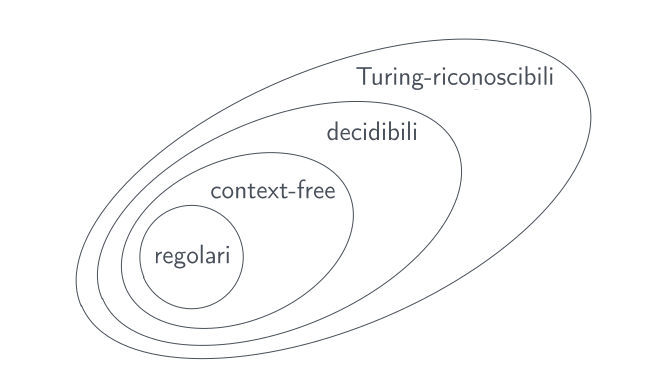
\includegraphics[scale=0.5]{img/rel_classi_linguaggi.png}
Queste non sono solo classi di linguaggi, ma anche \g{classi di capacità computazionale}. 
\newpage
\section{Indecidibilità}
\subsection{Metodo della diagonalizzazione}

Tale metodo è un metodo scoperto da Cantor nel 1873, e serve per confrontare le dimensioni di \g{insiemi infiniti}.

\g{due insiemi finiti hanno la stessa dimensione se gli elementi di un insieme possono essere accoppiati agli elementi dell'altro insieme}

\paragraph{Corrispondenze}
Abbiamo due insiemi $A$ e $B$ e una funzione $f:A\rightarrow B$ 
\begin{itemize}
	\item $f$ è \g{iniett} se non mappa mai elementi diversi nello stesso punto: $f(a)\neq f(b)$ ogniqualvolta che $a\neq b$ 
	\item $f$ è \g{suriettiva} se tocca ogni elemento di $B$: 
  	Per ogni $b\in B$ esiste $a\in A$ tale che $f(a)=b$ 
	\item Una funzione iniettiva e suriettiva è chiamata \g{biettiva}: è un modo per \g{accoppiare} elementi di $A$ con elementi di $B$ 
\end{itemize}
\paragraph{Definizione}
$A$ e $B$ hanno la \g{stessa cardinalità} se esiste una funzione \g{biettiva} $f:A\rightarrow B$ 

\subsection{Esempio: naturali vs numeri pari}
\begin{itemize}
	\item $\mathbb{N}=\{0,1,2,\dots\}$, insieme dei numeri naturali.
	\item $\mathbb{E} = \{0,2,4,\dots\}$, insieme dei numeri pari.
\end{itemize}
\g{Quale dei due insiemi è il più grande?}\\

\paragraph{Definizione di insieme numerabile} 
Un insieme è \g{numerabile} se è finito oppure la la stessa cardinalità di $\mathbb{N}$ 

\paragraph{Altri esempi}
\begin{itemize}
	\item $\mathbb{Q}$ è numerabile? 
	\item $\mathbb{R}$ è numerabile? 
	\item Dato un alfabeto finito $\Sigma$, $\Sigma^*$ è numerabile? 
	\item L'insieme di \g{tutte le macchine di Turing} è numerabile? 
	\item L'insieme di \g{tutte le sequenze binarie infinite} è numerabile? 
	\item Dato un alfabeto finito $\Sigma$, l'insieme di \g{tutti i linguaggi} su $\Sigma^*$ è numerabile? 
\end{itemize}

\paragraph{Corollario}
\begin{itemize}
	\item L'insieme di tutte le macchine di Turing è \g{numerabile} 
	\item L'insieme di tutti i linguaggi è \g{non numerabile} 
	\item \g{devono} esistere linguaggi non riconoscibili da una macchina di Turing 
\end{itemize}

\subsection{Un risultato fondamentale}
\textit{Esiste un problema specifico che è algoritmicamente \g{irrisolvibile}}
\begin{itemize}
	\item Problemi di interesse non solo teorico, ma anche pratico.
	\item Esempio: Verifica del software: 
\end{itemize}
Verificare che un programma è corretto non è risolvibile algoritmicamente 
\begin{theorem}
	$A_{TM}$ è indecidibile
\end{theorem}
$A_{TM}=\{\langle M,w\rangle\mid M$ è una TM che accetta la stringa $w\}$ 
\begin{itemize}
	\item \g{Chiarimento}: $A_{TM}$ è Turing-riconoscibile
	\item Conseguenza: i riconoscitori **sono più potenti** dei decisori
	\item $U=$ ``Su input $\langle M,w\rangle$, dove $M$ è una TM e $w$ una stringa: 
		1. Simula $M$ su input $w$ 
		2. Se la simulazione raggiunge lo stato di accettazione, \g{accetta}; se raggiunge lo stato di rifiuto, \textit{rifiuta}.''
	\item $U$ è un \g{riconoscitore}. Perché non è un \g{decisore}? 
\end{itemize}

\subsection{Macchina Universale di Turing}
$U$ è un esempio di \g{Macchina Universale di Turing} 
Introdotta da Alan Turing nel 1936, può simulare \g{qualsiasi macchina di Turing} a partire dalla sua descrizione. 

\begin{theorem}
	$A_{TM}$ è indecidibile
\end{theorem}
$A_{TM}= \{\langle M,w\rangle\mid M$ è una TM che accetta la stringa $W\}$ 
\paragraph{Dimostrazione}
\begin{itemize}
	\item Per contraddizione. Assumiamo $A_{TM}$ decidibile per poi trovare una contraddizione
	\item Supponiamo $H$ decisore per $A_{TM}$ 
	\item Cosa fa $H$ con input $\langle M,w\rangle$ ?
\end{itemize}
$H(\langle M,w\rangle)=$ \g{accetta} se $M$ accetta $w$, \textit{rifiuta} altrimenti
\begin{itemize}
\item Definiamo una TM $D$  che usa $H$ come subroutine 
\item $D=$ ``Su input $\langle M\rangle$, dove $M$ è una TM: 
	\begin{enumerate}
		\item Esegue $H$ su input $\langle M,\langle M\rangle\rangle$
		\item  Dà in output l'opposto dell'output di $H$, se $H$ accetta, \textit{rifiuta}; se $H$ rifiuta, \g{accetta} 
	\end{enumerate}
\item Cosa fa $D$ con input $\langle D\rangle$ ? 
$D(\langle D\rangle)=$ \g{accetta} se $D$ non accetta $\langle D\rangle$, \textit{rifiuta} altrimenti.
\end{itemize}
\g{Questa è una contraddizione!}

\paragraph{Comprendere la dimostrazione}
\begin{enumerate}
	\item H accetta $\langle M,w\rangle$ esattamente quando $M$ accetta $w$ 
		\begin{enumerate}
			\item  Banale: abbiamo assunto che $H$ esista e decida $A_{TM}$ 
			\item $M$ rappresenta **qualsiasi** TM e $w$ è una **qualsiasi** stringa 
		\end{enumerate}
	\item $D$ rifiuta $\langle M\rangle$ esattamente quando $M$ acetta $\langle M \rangle$ 
		\begin{enumerate}
			\item Cosa è successo a $w$? 
			\item $w$ è solo una stringa, come $\langle M \rangle$. Tutto ciò che stiamo facendo è definire quale stringa dare in input alla macchina. 
		\end{enumerate}
	\item $D$ rifiuta $\langle D\rangle$ esattamente quando $D$ accetta $\langle D\rangle$ \\
		 Questa è la contraddizione 
	\item Dove si usa la diagonalizzazione? 
\end{enumerate}

\subsection{Un linguaggio non Turing-riconoscibile}
\begin{itemize}
	\item Abbiamo visto che $A_{TM}$ è \g{Turing-riconoscibile} 
	\item Sappiamo che l'insieme di \g{tutte le TM} è \g{numerabile} 
	\item Sappiamo che l'insieme di \g{tutti i linguaggi} è \g{non numerabile} 
	\item Di conseguenza \g{deve} esistere un linguaggio non \g{Turing-riconoscibile} 
\end{itemize}

C'è ancora una cosa che dobbiamo fare prima di poter mostrare un linguaggio non \g{Turing-riconoscibile}.\\
Mostreremo che se un linguaggio e il suo complementare sono Turing-riconoscibili, allora il linguaggio è decidibile. \\
Un linguaggio è \g{co-Turing riconoscibile} se è il complementare di un linguaggio Turing-riconoscibile
\begin{theorem}
	Un linguaggio è decidibile se e solo se è Turing-riconoscibile e co-Turing riconoscibile.
\end{theorem}
\paragraph{Dimostrazione}
\begin{itemize}
	\item Dobbiamo dimostrare entrambe le direzioni 
	\item Se $A$ è decidibile, allora sia $A$ che $\overline{A}$ sono Turing-riconoscibili
		\begin{itemize}
			\item Il complementare di un linguaggio decidibile è decidibile! \end{itemize}
	\item Se $A$ e $\overline{A}$ sono Turing-riconoscibili, possiamo costruire un decisore per $A$ 
\end{itemize}

\subsection{$\overline{A_{TM}}$ non è Turing-riconoscibile}
Se il complementare di $A_{TM}$ fosse Turing-riconoscibile, allora $A_{TM}$ sarebbe decidibile.
Sappiamo che $A_{TM}$ non è decidibile, quindi il suo complementare non può essere Turing-riconoscibile! 
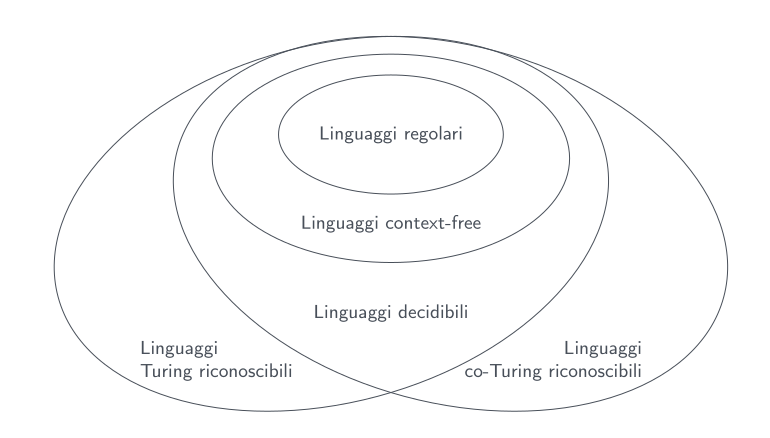
\includegraphics[scale=0.5]{img/linguaggi_diagramma.png}
\newpage
\section{Riducibilità}
Vediamo un altro problema indecidibile
\paragraph{Il problema della fermata}
$HALT_{TM}=\{\langle M,w\rangle\mid M$ è una TM che si ferma su input $w\}$ 
Come possiamo dimostrare che $HALT_{TM}$ è indecidibile? 
Possiamo provare con la \g{diagonalizzazione} 
Sappiamo che $A_{TM}$ è indecidibile: \g{possiamo usare questo fatto per semplificare la dimostrazione?}

\paragraph{Riducibilità}
\begin{itemize}
	\item Una \g{riduzione} è un modo per trasformare un problema in un altro problema
	\item Una soluzione al secondo problema può essere usata per \g{risolvere il primo problema} 
	\item Se $A$ è riducibile a $B$, e $B$ è decidibile, allora $A$ è \g{decidibile} 
	\item Se $A$ è riducibile a $B$, e $A$ è decidibile, allora $A$ è \g{decidibile} 
\end{itemize}
\subsection{Dimostrazione per riduzione }
Queste dimostrazioni sono usate per dimostrare che un problema è indecidibile: 
\begin{enumerate}
	\item **Assumi** che $B$ sia decidibile
	\item **Riduci** $A$ al problema $B$ 
		\begin{itemize}
			\item costruisci una TM che usa $B$ per risolvere $A$ 
		\end{itemize}
	\item si $A$ è indecidibile, allora questa è una \g{contraddizione} 
	\item L'assunzione è sbagliata e $B$ è indecidibile
\end{enumerate}

\subsection{Il problema del vuoto}
$E_{TM} = \{\langle M\rangle\mid M$ è una TM tale che $L(M)=\varnothing\}$ 
\begin{itemize}
	\item La dimostrazione è per contraddizione e riduzione di $A_{TM}$ 
	\item Chiamiamo $R$ la TM che decide $E_{TM}$ 
	\item Useremo $R$ per costruire la TM $S$ che decide $A_{TM}$ 
\end{itemize}

\subsection{Stabilire se un linguaggio è regolare}
$REGULAR_{TM} = \{\langle M\rangle\mid M$ è una TM tale che $L(M)$ è regolare $\}$ 
\begin{itemize}
	\item La dimostrazione è per contraddizione e riduzione di $A_{TM}$ 
	\item Chiamiamo $R$ la TM che decide $REGULAR_{TM}$ 
	\item Useremo $R$ per costruire la TM $S$ che decide $A_{TM}$ 
	\item Capire come possiamo usare $R$ per implementare $S$ è meno ovvio di prima 
\end{itemize}

\subsection{Il problema dell'equivalenza}
$EQ_{TM} = \{\langle M_1,M_2\mid M_1, M_2$ TM tali che $L(M_1)=L(M_2)\}$ 
\begin{itemize}
	\item La dimostrazione è per contraddizione e riduzione di $E_{TM}$ (problema del vuoto)
	\item Chiamiamo $R$ la TM che decide $EQ_{TM}$ 
	\item Useremo $R$ per costruire la TM $S$ che decide $E_{TM}$ 
\end{itemize}

\subsection{Riducibilità mediante funzione}
Trasforma istanze del problema $A$ in istanze del problema $B$ mediante una \g{funzione calcolabile} 
\begin{itemize}
	\item Chiarisce e formalizza la riducibilità
		\paragraph{Definizione}
		$f:\Sigma^*\rightarrow\Sigma^*$ è una \g{funzione calcolabile} se esiste una TM $M$ che su input $w$, termina la computazione avendo solo $f(w)$ sul nastro
	\item Le operazioni aritmetiche sugli interi sono funzioni calcolabili
	\item Le trasformazioni di macchine di Turing possono essere funzioni calcolabili
\end{itemize}

Un linguaggio $A$ è \g{riducibile mediante funzione} al linguaggio $B$ $(A\leq_m B)$, se esiste una \g{funzione calcolabile} $f:\Sigma^*\rightarrow\Sigma^*$ tale che 
Per ogni $w:w\in A$ se e solo se $f(w)\in B$ \\
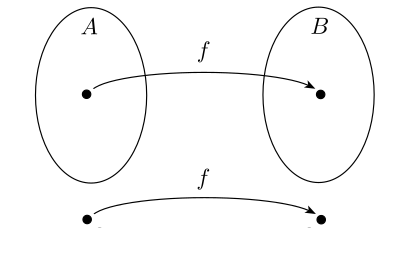
\includegraphics[scale=0.5]{img/funzione_riduzione.png}\\
$f$ è la **riduzione** da $A$ a $B$ 

Se esiste una \g{riduzione} da $A$ e $B$, possiamo risolvere $A$ usando una soluzione per $B$: \\
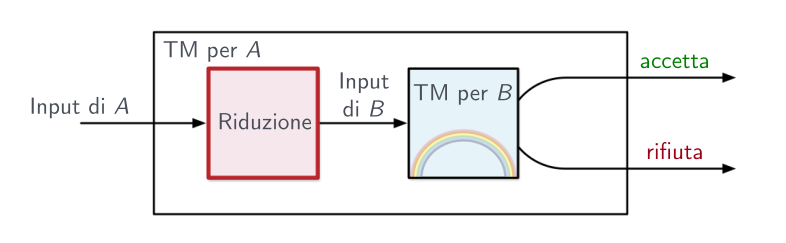
\includegraphics[scale=0.5]{img/schema_riducibilita.png}
\subsection{Proprietà delle riduzioni}
\paragraph{Teorema}
Se $A\leq_m B$ e $B$ è ???, allora $A$  è ??? 
\paragraph{Teorema}
Se $A\leq_m B$ e $A$ è  allora $B$ è ??? 

\subsection{Il problema della fermata(2)}
$HALT_{TM}=\{\langle M,w\rangle\mid M$ è una TM che si ferma su input $w\}$ 
\begin{itemize}
	\item Possiamo dimostrare che $A_{TM}\leq_m HALT_{TM}$ ? 
	\item Qual è l'input della funzione di riduzione? 
	\item Qual è l'output? 
	\item Quali proprietà devono rispettare? 
\end{itemize}
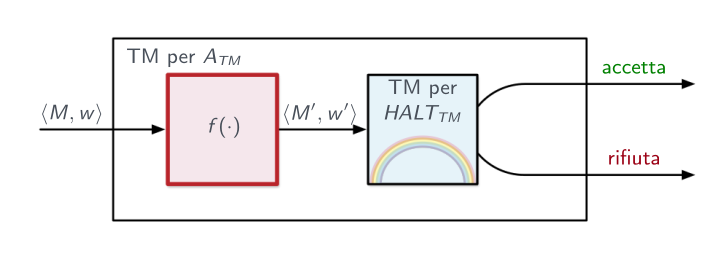
\includegraphics[scale=0.5]{img/schema_halt.png}\\
$M$ accetta $w$ se e solo se $M'$ si ferma su $w'$ 
\subsection{Il problema dell'equivalenza(2)}
$$EQ_{TM}=\{\langle M_1, M_2\rangle\mid L(M_1)=L(M_2)\}$$
\begin{itemize}
	\item Possiamo dimostrare che $E_{TM}\leq_m EQ_{TM}$ ?
	\item Qual è l'input della funzione di riduzione? 
	\item Qual è l'output? 
	\item Quali proprietà devono rispettare? 
\end{itemize}
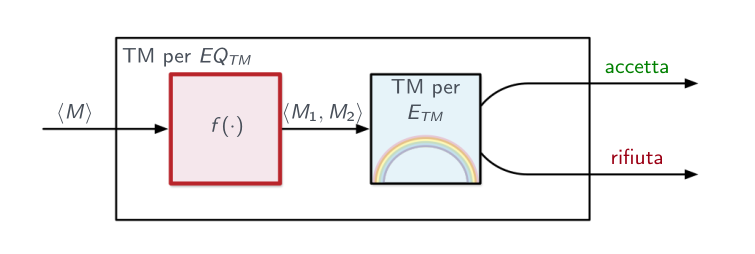
\includegraphics[scale=0.5]{img/schema_eq_tm.png}
$L(M)=\varnothing$ se e solo se $L(M_1)=L(M_2)$ 

\subsection{Il problema del vuoto(2)}
$E_{TM}=\{\langle M\rangle\mid M$ è una TM tale che $L(M)=\varnothing\}$ 
\begin{itemize}
	\item Possiamo dimostrare che $A_{TM}\leq_m E_{TM}$ ?
	\item Qual è l'input della funzione di riduzione? 
	\item Qual è l'output? 
	\item Quali proprietà devono rispettare? 
\end{itemize}
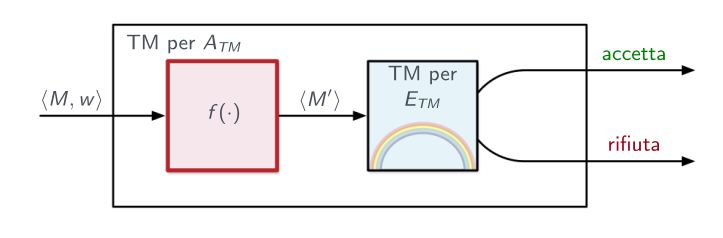
\includegraphics[scale=0.5]{img/schema_atm_etm.png}
$M$ accetta $w$ se e solo se $L(M')=\varnothing$ 
\begin{center}
	{\Large STOP!!!}
\end{center}
\g{Non sappiamo come ridurre il problema dell'accettazione al problema del vuoto!}
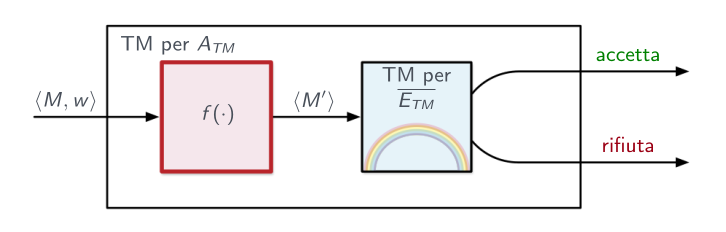
\includegraphics[scale=0.5]{img/schema_atm_etm_2.png}
$M$ accetta $w$ se e solo se $L(M') \neq \varnothing$ 
\paragraph{Proprietà delle riduzioni (2)}
\paragraph{Teorema}
Se $A\leq_m B$ e $B$ è ???, allora $A$  è ??? 
\paragraph{Teorema}
Se $A\leq_m B$ e $A$ è ???  allora $B$ è ??? 
\newpage
\section{Complessità di tempo}
\subsection{Misure di Complessità}
Comsideriamo il linguaggio $A=\{0^k1^k\mid k \geq 0\}$
\begin{itemize}
  \item Che tipo di linguaggio è?
  \item È \g{decidibile}?
  \item Quanto \g{tempo} serve ad una TM a nastro singolo per decidere questo 
    linguaggio?
\end{itemize}
\paragraph{Definizione}
\begin{itemize}
  \item Sia $M$ una TM \g{deterministica} che si \g{ferma} su tutti gli input
  \item Il \g{tempo di eseguzione} (o \g{complessità di tempo}) di $M$ è
    la funzione $f:\mathbb{N} \mapsto\mathbb{N}$ tale che $f(n)$ è 
    il numero massimo di passi che $M$ utilizza su un input di lunghezza $n$.
  \item Se $f(n)$ è il tempo di esecuzione di $M$, diciamo che $M$ è una TM
    \g{di tempo $f(n)$}
  \item Useremo $n$ per rappresentare la \g{lunghezza dell'input}
  \item Ci interesseremo dell'\g{analisi del caso pessimo}
\end{itemize}
\subsection{Notazione $O$-grande}
\begin{itemize}
  \item \g{Analisi asintotica}: valuta il tempo di esecuzione su input grandi 
  \item Considera solo il \g{termine di ordine maggiore} e \g{ignora i coefficienti}
    \begin{definition}
      Date due funzioni $f,g$, diciamo che $f(n) = O(g(n))$ se esistono interi positivi
      $c, n_0$ tali che per ogni $n\geq n_0$
      \begin{displaymath}
        f(n)\leq c g(n)
      \end{displaymath}
      $g(n)$ è un \g{limite superiore asintotico} per $f(n)$ 
    \end{definition}
\end{itemize}
\subsection{Analisi di complessità}
Analizziamo questa TM per $A=\{0^k1^k\mid g\geq 0\}$\\
$M_1 =$ ``Su input $w$:
\begin{enumerate}
  \item Scorrere il nastro e \textit{rifiuta} se trova uno 0 a destra di un 1
  \item Ripete finché il nastro contiene almeno uno 0 e un 1
  \item Scorre il nastro cancellando uno 0 e un 1
  \item Se rimane almeno uno 0 dopo che ogni 1 è stato cancellato, 
    o se rimane almeno un 1 dopo che ogni 0 è stato cancellato, \textit{rifiuta}. 
    Altrimenti, se non rimangono né 0 né 1 sul nastro, \g{accetta}''
\end{enumerate}
\subsection{Classi di complessità di tempo}
\begin{definition}
  Sia $t:\mathbb{N}\mapsto\mathbb{N}$ una funzione\\
  La \g{classe di complessità di tempo $TIME(T(N))$} è l'insieme di tutti i 
  linguaggi che sono \g{decisi} da una \g{TM in tempo $O(t(n))$}
  \begin{itemize}
    \item Questo è diverso dalle classi di linguaggi discusse in precedenza, 
      che si concentravano sulla \g{computabilità}
    \item Questa classificazione si concentra sul \g{tempo necessario}
      per decidere il linguaggio.
  \end{itemize}
\end{definition}
\paragraph{Possiamo fare di meglio?} Dall'analisi che abbiamo fatto, sappiamo che 
$$ A=\{0^k1^k\mid k\geq 0\}$$
appartiene alla classi di complessità di tempo \g{$TIME(n^2$}, perché $M_1$ 
decide $A$ in tempo $O(n^2)$
\paragraph{MA} Esiste una macchina che decide $A$ in modo \g{asintoticamente più veloce}?
\paragraph{Miglioriamo $M_1$}\g{Idea}: cancelliamo metà degli 0 e metà degli 1 ad
ogni scansione
$M_2=$ ``Su input $W$:
\begin{enumerate}
  \item Scorre il nastro e \g{rifiuta} se trova uno 0 a destra di un 1
  \item Ripete finché il nastro contiene almeno uno 0 ed un 1
  \item Scorre il nastro e controlla se il numero totale di 0 e 1 rimasti
    è pari o dispari. Se è dispari, \textit{rifiuta}
  \item Scorre il nastro, cancellando prima ogni secondo 0 a partire dal primo
    0, poi cancellando ogni secondi 1 a partire dal primo 1.
  \item se nessuno 0 e nessun 1 rimangono sul nastro \g{acetta}. 
    Altrimenti \textit{rifiuta}
\end{enumerate}
\paragraph{Possiamo fare ancora meglio?}
\begin{itemize}
  \item Possiamo trovare una TM che decide $A$ in $O(n)$?
  \item \g{Problema}: non esiste una TM \g{a nastro singolo} che è in grado di decidere 
    $A$ in tempo $O(n)$.
  \item Possiamo farlo se la TM \g{ha un secondo nastro}
  \item \g{Importante}: la complessità di tempo dipende dal \g{modello di calcolo}
  \item La \g{Tesi di Church-Turing} implica che tutti i modelli di calcolo ``ragionevoli''
    siano equivalenti.
  \item \g{in pratica}: discuteremo qunto questa differenza sia importante (o meno) 
    per il nostro sistema di classificazione più avanti. 
\end{itemize}
\g{Idea}: usiamo il secondo nastro per contare 0 e 1
$M_2 =$ ``Su input $w$:
\begin{itemize}
  \item Scorre il nastro 1 e \textit{rifiuta} se trova uno 0 a destra di un 1
  \item Scorre i simboli 0 sul nastro 1 fino al primo 1. 
    Contemporaneamente, copia ogni 0 sul nastro 2.
  \item Scorre i simboli 1 sul nastro 1 fino alla fine dell'input. 
    Per ogni 1 letto sul nastro 1, cancella uno 0 sul nastro 2.
    Se ogni 0 è stato cancellato prima di aver letto tutti gli 1, \textit{rifiuta}
  \item Se tutti gli 0 sono stati cancellati, \g{accetta}. 
    Se rimane qualche 0, \textit{rifiuta}
\end{itemize}
\subsection{Relazione di complessità tra modelli}
\subsubsection{Singolo nastro vs. Multinastro}
\begin{theorem}
  Sia $t(n)$ una funzione tale che $t(n) \leq n$. Ogni TM \g{multinastro}
  di tempo $t(n)$ ammette una TM equivalente a \g{nastro singolo} di tempo 
  $O(t^2(n))$.
\end{theorem}
\begin{itemize}
  \item Ricordiamo la dimostrazione di come convertire una TM da multinastro 
    a nastro singolo.
    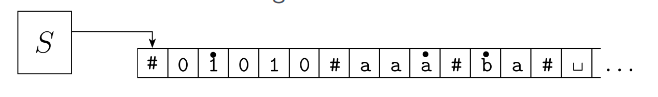
\includegraphics[scale=0.5]{img/nastro.png}
  \item Dobbiamo determinare quanto tempo ci vuole per simulare ogni passo 
    della macchina multinastro sulla TM a nastro singolo. 
\end{itemize}
\subsubsection{TM non deterministiche}
\begin{theorem}
  Sia $N$ una TM non deterministica che è anche un \g{decisore}. 
  Il \g{tempo di esecuzione} di $N$ è la funzione $f: \mathbb{N}\mapsto \mathbb{N}$
  tale che $f(n)$ è il massimo numero di passi che $N$ usa per ognuno dei rami di computazione, 
  su input di lunghezza $n$. 
\end{theorem}
\paragraph{Nota Bene} la definizione di tempo di esecuzione per le TM non deterministiche 
non è destinato a corrispondere ad un qualche dispositivo di calcolo reale. 
È uno strumento teorico che utilizziamo per comprendere i problemi computazionali.\\
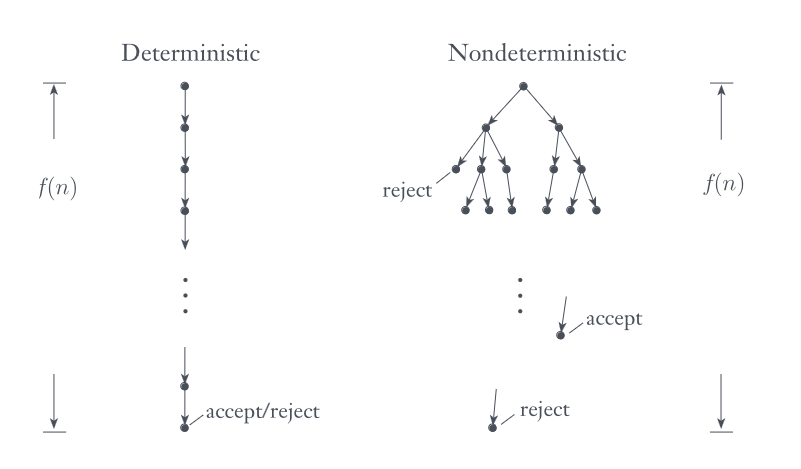
\includegraphics[scale=0.5]{img/tm_non_deterministiche.png}
\subsubsection{Determinismo vs. Non determinismo}
\begin{theorem}
  Sia $t(n)$ una funzione tale che $t(n)\leq n$. Ogni TM \g{non deterministica}
  di tempo $t(n)$ ammette una TM equivalente a \g{nastro singolo} di tempo 
  $2^{O(t(n))}$.
\end{theorem}
\paragraph{Dimostrazione}
\begin{itemize}
  \item Sia $N$ una TM non deterministica di tempo $t(n)$ 
  \item Costruiamo una TM deterministica $D$ che simula $N$. 
  \item $D$ è una TM \g{multinastro}. Qual è la complessità quando viene 
    convertita in una TM a nastro singolo? 
\end{itemize}
\newpage
\section{Classe P}
Riassunto: 
\begin{itemize}
  \item Differenza di tempo \g{polinomiale} tra TM a nastro singolo e multi-nastro
  \item Differenza di tempo \g{esponenziale} tra TM deterministichee non deterministiche
\end{itemize}
Una differenza \g{polinomiale} è considerata piccola
\begin{itemize}
  \item Tutti i modelli di calcolo deterministici ``ragionevoli'' sono 
    \g{polinomialmente equivalenti}
  \item ``Ragionevole'' è definito in modo approssimativo, ma include
    modelli che assomigliano molto ai computer reali
\end{itemize}
Una differenza \g{esponenziale} è considerata grande
\begin{definition}
  $P$ è l classe di linguaggi che sono decidibili in \g{tempo polinomiale}
  da una TM deterministica a singolo nastro
  \begin{displaymath}
    P=\underset{k}{\bigcup}TIME(n^k)
  \end{displaymath}
\end{definition}
\begin{itemize}
  \item $P$ è invariante per i modelli di calcolo \g{polinomialmente equivalenti}
    ad una TM deterministica
  \item $P$ corrisponde approssimativamente ai problemi che sono 
    \g{realisticamente risolvibili} da un computer
\end{itemize}
Per dimostrare che un problema/algoritmo è in $P$ 
\begin{itemize}
  \item Descrivi l'algoritmo per fasi numerate 
  \item Dai un limite superiore polinomiale al numero di fasi che l'algoritmo 
    esegue per un input di lunghezza $n$ 
  \item Assicurati che ogni fase possa essere completata in tempo polinomiale
    su un modello di calcolo deterministico ragionevole
  \item L'input deve essere codificato in modo ragionevole
\end{itemize}
\subsection{Due problemi in $P$}
\begin{description}
  \item[Raggiungibilità di un grafo] 
    $PATH = \{\langle G,s,t\rangle\mid G\textrm{ grafo che contiene un cammino da} s \textrm{ a }t\}$
  \item[Numeri relativamente primi]
    $RELPRIME = \{(x,y)\mid 1\textrm{ è il massimo comun divisore di }x \textrm{ e }y\}$
\end{description}
\begin{theorem}
  ogni linguaggi context-free è un elemento in $P$ 
\end{theorem}
\begin{itemize}
  \item Abbiamo dimostrato che ogni CFL è \g{decidibile}
    \begin{itemize}
      \item L'algoritmo nella dimostrazione è \g{esponenziale}
    \end{itemize}
  \item La soluzione polinomiale usa la \g{programmazione dinamica}
  \item La complessità è $O(n^3)$ 
\end{itemize}

\newpage
\section{La classe NP}
\subsection{Giochiamo a Domino}
Disponete in file le \g{tessere del domino} che vi sono state consegnate in modo da 
usare tutte le tessere. 
% immagine
\g{È un problema facile o difficile da risolvere?}
\begin{definition}
  Un problema è \g{trattabile} (facile) se esiste un \g{algoritmo efficiente}
  per risolverlo
\end{definition}
\begin{itemize}
  \item Gli algoritmi efficienti sono \g{algoritmi con complessità polinomiale}, 
    il loro tempo di esecuzione è $O(n^2)$ per qualche costante $k$.
  \item Avere complessità polinomiale è una \g{condizione minima} per considerare 
    un algoritmo efficiente
  \item Un algoritmo con complessità più che polinomiale (per esempio esponenziale)
    è un algoritmo \g{non efficiente} perché non è scalabile. 
\end{itemize}
\subsection{Mostriamo che Domino[1] è trattabile}
\paragraph{Obiettivo} Trovare un algoritmo polinomiale per \g{Domino[1]}
\begin{itemize}
  \item Formulazione del problema in termini di \g{linguaggio}
  \item Definizione di una Macchina di Turing che lo \g{decide}
  \item Analisi di \g{complessità} della macchina di Turing
    (o dell'algoritmo)
\end{itemize}
\subsection{Un linguaggio e una riduzione}
$D_1=\{\langle B\rangle\mid B\textrm{ 
  è un insieme di tessere del domino, ed esiste un allineamento 
  che usa tutte le tessere
  }\}$
\begin{itemize}
  \item Usiamo una \g{Riduzione mediante funzione} per trovare l'algoritmo
    polinomiale.
  \item Riduciamo $D_1$ ad un \g{problema su grafi}
  \item ... per il quale sappiamo che \g{esiste un algoritmo polinomiale}
\end{itemize}
\subsection{Dalle tessere al grafo}
\begin{definition}
  Un grafo (non orientato) è una coppia (V,E) dove:
 \begin{itemize}
   \item $V = \{v_1, v_2,\dots,v_n\}$ è un insieme finito e non vuoto di \g{vertici}
   \item $E\subseteq\big\{\{u,v\}\mid u,v\in V\big\}$ è un insieme di 
     \g{coppie non ordinate}
     ognuna delle quai corrisponde ad un \g{arco} del grafo.
 \end{itemize} 
\end{definition}
\paragraph{Grafo del dominio}
\begin{itemize}
  \item \g{Vertici}: i numeri che si trovano sulle tessere
    \begin{itemize}
      \item $V = \{\epsdice{1},\epsdice{2},\epsdice{3},\epsdice{4}\}$
    \end{itemize}
  \item \g{Archi}: le tessere del domino
    \begin{itemize}
      \item $E =  \{\epsdice{3}\epsdice{4}, \epsdice{1}\epsdice{2},
        \epsdice{4} \epsdice{2},\epsdice{4} \epsdice{1}, 
                   \epsdice{3} \epsdice{2} \}$
    \end{itemize}
\end{itemize}
\subsection{Dominio[1] è un problema su grafi!}
\g{Camino Euleriamo}: percorso di un grafo che attraversa \g{tutti gli archi}
una sola volta.
\paragraph{Il problema del Cammino Euleriano}
\[
  EULER = \{\langle G\rangle\mid \textrm{
    è un grafo che possiede un cammino Euleriano
  }\}
\]
\begin{itemize}
  \item $EULER$ è un problema classico di \g{teoria dei grafi}
  \item Esistono \g{algoritmo polinomiali} per risolverlo.
\end{itemize}
\subsection{Algoritmo di Fleury}
\begin{itemize}
  \item Scegliere un vertice con \g{grado dispari} 
    (un vertice qualsiasi se tutti pari)
  \item Scegliere un arco tale che la sua cancellazione \g{non sconnetta il grafo}
  \item \g{Passare} al vertice nell'altra estremità dell'arco scelto.
  \item \g{Cancellare} l'arco del grafo
  \item \g{Ripetere} i tre precedenti finché non eliminate tutti gli archi
\end{itemize}
\paragraph{Complessità} Su un grafo con $n$ archi, l'algoritmo di Fleury impiega 
tempo $O(n^2)$ 
\subsection{Complessità di Domino[1]}
\begin{itemize}
  \item L'algoritmo di Fleury risolve $EULER$ in tempo \g{polinomiale}
  \item La riduzione ci dice che $D_1 \leq_m EULER$ 
  \item Quanto tempo serve per risolvere il problema $D_1$? 
\end{itemize}
\subsection{Giochiamo a domino[2]}
Disponete in file le tessere del domino che vi sono state consegnate in modo che 
\g{ogni numero} compaia \g{esattamente due volte}
(potete usare meno tessere di quelle che avete)
\g{È un problema facile o difficile da risolvere?}
\subsubsection{Una riduzione in senso opposto!}
\[
  D_2 = \{\langle B\rangle\mid B\textrm{ insieme di tessere del domino, ed } \exists 
 \textrm{ allineamento dove ogni numero compare 2 volte}\}
\]
\begin{itemize}
  \item \g{Corcuito Hamiltoniano}: ciclo nel grafo che attraversa \g{tutti i vertici}
    una sola volta
\end{itemize}
\begin{definition}[Il problema del Circuito Hamiltoniano]
  $HAMILTON =\{\langle G\rangle\mid G\textrm{ è un grafo con un circuito Hamiltoniano}\}$
\end{definition}
Come facciamo a dinostrare che $HAMILTON \leq_m D_2$? 
\subsection{$HAMILTON$ è un problema difficile!}
\begin{itemize}
  \item Il problema del \g{circuito Hamiltoniano} è un problema classico di 
    \g{teoria dei grafi}
  \item Un \g{algoritmo polinomiale} per risolverlo \g{non è mai stato trovato}
  \item Se qualcuno mi dà una \g{possibile soluzione}, è \g{facile verificare} 
    se è corretta
\end{itemize}
\subsection{Problemi trattabili e probemi intrattabili}
\begin{itemize}
  \item I problemi per i quali esiste un algoritmo polinomiale vengono considerati
    \g{trattabili}
  \item quelli che richiedono un algoritmo più che polinomiale sono detti \g{intrattabili}
  \item Sappiamo che ci sono problemi che non possono essere risolti da \g{nessun algoritmo}:
    \begin{itemize}
      \item ``Hamilton Problem'' di Turing.
    \end{itemize}
  \item Ci sono problemi che richiedono un tempo \g{esponenziale}
    \begin{itemize}
      \item Il gioco della Torre di Hanoi
    \end{itemize}
\end{itemize}
\begin{center}
  \g{Stabilire con precisione qual'è il confine tra problemi trattabili 
  ed intrattabili è piuttosto difficile} 
\end{center}
\subsection{P vs NP}
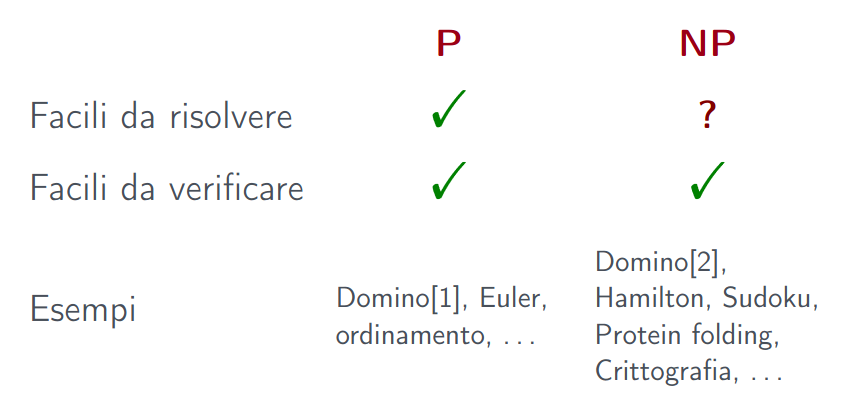
\includegraphics[scale=0.5]{img/pvsnp.png}

% SCHIFEZZE DELLA ISSUE #34 DI GITHUB

\subsection{Verificatori}
\begin{definition}
  Un \g{verificatore} per il linguaggio $A$ è un algoritmo $V$ tale che 
  \begin{displaymath}
    A+\{w\mid V\textrm{ accetta } \langle w,c\rangle\textrm{ per qualche stringa }c\}
  \end{displaymath}
\end{definition}
\begin{itemize}
  \item Il verificatore usa \g{ulteriori informazioni} per stabilire se $w$ appartiene 
    al linguaggio
  \item questa informazione è il \g{certificato} c
\end{itemize}
\subsection{Problemi P ed NP} 
\begin{description}
  \item [P] è la classe dei linguaggi che possono essere \g{decisi} da una 
    macchina di Turing deterministica che inpiega \g{tempo polinomiale}
  \item [NP] è la classe dei linguaggi che ammettono un \g{verificatore}
    che impiega \g{tempo polinomiale}
  \item [Equivalente] è la classe dei linguaggi che possono essere decisi da una macchina 
    di Turing \g{non deterministica} che impiega \g{tempo polinomiale}.
\end{description}
\subsubsection{Due problemi in P}
\paragraph{Raggiungibilità di un grafo}\nin

$PATH=\{\langle G,s,t\rangle\mid G \textrm{ grafo che contiene un cammino da } s \textrm{ a }t\}$
\paragraph{Numeri relativamente primi}\nin

$RELPRIME = \{\langle x,y\rangle\mid 1 \textrm{ è il massimo comun divisore di }x\textrm{ e }y\}$
\subsubsection{Due problemi in NP}
\paragraph{Problema del circuito Hamiltoniano}\nin

$HAMILTON =\{\langle G\rangle\mid G\textrm{ è un grafo con un circuito Hamiltoniano}\}$
\paragraph{Numeri composti}\nin

$COMPOSITES = \{\langle x\rangle\mid x = pq\textrm{, per gli interi }p,q>1\}$
\newpage

% \input{sections/6_successioni.tex}\newpage
% \input{sections/7_cardinalita_di_insiemi.tex}\newpage
% \input{sections/8_topologia_retta_euclidea.tex}\newpage
% \input{sections/9_punti_accumulazione.tex}\newpage
% \input{sections/10_insiemi_chiusi.tex}\newpage
% \input{sections/11_insiemi_aperti_e_chiusi.tex}\newpage
% \input{sections/12_limiti_per_funzioni.tex}\newpage

\end{document}

